\documentclass[11pt,a4paper]{article}
\usepackage[margin=2.5cm]{geometry}
\usepackage{iohk}
\usepackage{microtype}
\usepackage{mathpazo} % nice fonts
\usepackage{amsmath}
\usepackage{amssymb}
\usepackage{latexsym}
\usepackage{mathtools}
\usepackage{stmaryrd}
\usepackage{extarrows}
\usepackage{slashed}
\usepackage[colon]{natbib}
\usepackage[unicode=true,pdftex,pdfa,colorlinks=true]{hyperref}
\usepackage{xcolor}
\usepackage[capitalise,noabbrev,nameinlink]{cleveref}
\usepackage{float}
\floatstyle{boxed}
\restylefloat{figure}
\usepackage{listings} % for code blocks.
%%
%% Package `semantic` can be used for writing inference rules.
%%
\usepackage{semantic}
%% Setup for the semantic package
\setpremisesspace{20pt}
\usepackage{tikz}
\usetikzlibrary{decorations.pathreplacing, positioning, arrows.meta, calc}
% For drawing simple diagrams involving arrows between LaTeX symbols
\usepackage{tikz-cd}

%%
%% Types
%%
\newcommand{\Bool}{\type{Bool}}
\newcommand{\Tx}{\type{Tx}}
\newcommand{\Ix}{\type{Ix}}
\newcommand{\TxId}{\type{TxId}}
\newcommand{\Addr}{\type{Addr}}
\newcommand{\UTxO}{\type{UTxO}}
\newcommand{\Value}{\type{Value}}
\newcommand{\Lovelace}{\type{Lovelace}}
%% Adding witnesses
\newcommand{\TxIn}{\type{TxIn}}
\newcommand{\TxOut}{\type{TxOut}}
\newcommand{\VKey}{\type{VKey}}
\newcommand{\SKey}{\type{SKey}}
\newcommand{\Hash}{\type{Hash}}
\newcommand{\SkVk}{\type{SkVk}}
\newcommand{\Sig}{\type{Sig}}
\newcommand{\Data}{\type{Data}}
%% Adding delegation
\newcommand{\Epoch}{\type{Epoch}}
\newcommand{\VKeyGen}{\type{VKey_G}}
%% Blockchain
\newcommand{\Gkeys}{\var{G_{keys}}}
\newcommand{\Block}{\type{Block}}
\newcommand{\CEEnv}{\type{CEEnv}}
\newcommand{\CEState}{\type{CEState}}
\newcommand{\BDEnv}{\type{BDEnv}}
\newcommand{\BDState}{\type{BDState}}
\newcommand{\Slot}{\type{Slot}}
\newcommand{\SlotCount}{\type{SlotCount}}

%%
%% Functions
%%
\newcommand{\txins}[1]{\fun{txins}~ \var{#1}}
\newcommand{\txid}[1]{\fun{txid}~ \var{#1}}
\newcommand{\txouts}[1]{\fun{txouts}~ \var{#1}}
\newcommand{\values}[1]{\fun{values}~ #1}
\newcommand{\balance}[1]{\fun{balance}~ \var{#1}}
%% UTxO witnesses
\newcommand{\inputs}[1]{\fun{inputs}~ \var{#1}}
\newcommand{\wits}[1]{\fun{wits}~ \var{#1}}
\newcommand{\verify}[3]{\fun{verify} ~ #1 ~ #2 ~ #3}
\newcommand{\sign}[2]{\fun{sign} ~ #1 ~ #2}
\newcommand{\serialised}[1]{\llbracket \var{#1} \rrbracket}
\newcommand{\addr}[1]{\fun{addr}~ \var{#1}}
\newcommand{\hash}[1]{\fun{hash}~ \var{#1}}
\newcommand{\txbody}[1]{\fun{txbody}~ \var{#1}}
\newcommand{\txfee}[1]{\fun{txfee}~ \var{#1}}
\newcommand{\minfee}[2]{\fun{minfee}~ \var{#1}~ \var{#2}}
% wildcard parameter
\newcommand{\wcard}[0]{\underline{\phantom{a}}}
%% Adding ledgers...
\newcommand{\utxo}[1]{\fun{utxo}~ #1}
%% Delegation
\newcommand{\delegatesName}{\fun{delegates}}
\newcommand{\delegates}[3]{\delegatesName~#1~#2~#3}
\newcommand{\dwho}[1]{\fun{dwho}~\var{#1}}
\newcommand{\depoch}[1]{\fun{depoch}~\var{#1}}
%% Delegation witnesses
\newcommand{\dbody}[1]{\fun{dbody}~\var{#1}}
\newcommand{\dwit}[1]{\fun{dwit}~\var{#1}}
%% Blockchain
\newcommand{\bwit}[1]{\fun{bwit}~\var{#1}}
\newcommand{\bslot}[1]{\fun{bslot}~\var{#1}}
\newcommand{\bbody}[1]{\fun{bbody}~\var{#1}}
\newcommand{\bdlgs}[1]{\fun{bdlgs}~\var{#1}}
%% Set notation
\newcommand\Set[2]{\{\,#1\mid#2\,\}}

%% For properties
\newcommand{\txs}{\ensuremath{\mathcal{T}}}
\newcommand{\transtar}[2]{\xlongrightarrow[\textsc{#1}]{#2}\negthickspace^{*}}
\newcommand{\biguo}[1]{\ensuremath{\underset{#1}{\underrightarrow\bigcup}}}

%\includeonly{update-mechanism, delegation, blockchain-interface}

%% Parameters that control floats placement. See https://robjhyndman.com/hyndsight/latex-floats/
\setcounter{topnumber}{2}
\setcounter{bottomnumber}{2}
\setcounter{totalnumber}{4}
\renewcommand{\topfraction}{0.85}
\renewcommand{\bottomfraction}{0.85}
\renewcommand{\textfraction}{0.15}
\renewcommand{\floatpagefraction}{0.7}

\newtheorem{definition}{Definition}
\newtheorem{prop}{Property}

\begin{document}

\hypersetup{
  pdftitle={A Formal Specification of the Cardano Ledger},
  breaklinks=true,
  bookmarks=true,
  colorlinks=false,
  linkcolor={blue},
  citecolor={blue},
  urlcolor={blue},
  linkbordercolor={white},
  citebordercolor={white},
  urlbordercolor={white}
}

\title{A Formal Specification of the Cardano Ledger}

\author{Jared Corduan  \\ {\small \texttt{jared.corduan@iohk.io}} \\
   \and Polina Vinogradova \\ {\small \texttt{polina.vinogradova@iohk.io}} \\
   \and Matthias G\"udemann  \\ {\small \texttt{matthias.gudemann@iohk.io}}}

%\date{}

\maketitle

\begin{abstract}
This documents defines the rules for extending a ledger with transactions.
The transactions will affect both UTxO and stake delegation.
It is intended to serve as the specification for random generators of transactions
which adhere to the rules presented here.
\end{abstract}

\section*{List of Contributors}
\label{acknowledgements}

Nicol\'as Arqueros,
Nicholas Clarke,
Duncan Coutts,
Ruslan Dudin,
Sebastien Guillemot,
Vincent Hanquez,
Ru Horlick,
Michael Hueschen,
Philipp Kant,
Jean-Christophe Mincke,
Damian Nadales,
Nicolas Di Prima.


\tableofcontents
\listoffigures

This document is a formal specification of the functionality of the ledger
on the blockchain. The blockchain layer of the
protocol and the interaction between the ledger and the blockchain
layer is presented in a separate document, see~\cite{shelley_consensus}. The details of the
background and the larger context
for the design decisions formalized in this document are presented
in~\cite{delegation_design}

In this work,
we present important properties any implementation of the ledger must have.
Specifically, we model the following aspects
of the functionality of the ledger on the blockchain:

\begin{description}
\item[Preservation of value] relationship between the total value of input and
  outputs in a new transaction, and the unspent outputs.
\item[Witnesses] authentication of parts of the transaction data by means of
  cryptographic entities (such as signatures and private keys) contained in
  these transactions.
\item[Delegation] validity of delegation certificates, which delegate
  block-signing rights.
\item[Stake] staking rights associated to an address.
\end{description}

While the blockchain protocol is a reactive system driven by the arrival
of blocks causing updates to the ledger, the formal description is a collection
of rules which is a
static description of what a \textit{valid ledger} is. The specifics of the
semantics we use to define and apply
the rules we present in this document are explained in detail in
\cite{small_step_semantics}. A valid ledger state can only
reached by applying a sequence of inference rules, and any valid ledger state
is reachable by applying some sequence of these rules.

The structure of the rules we give here is such that their application is
deterministic. That is, given a specific initial state and relevant environmental
constants, there is no ambiguity
about which rule should be applied at any given time (i.e. which state
transition is allowed take place). This is an important property which reflects
the reality of the implementation - the blockchain evolves in a particular way
given some user activity and the passage of time, and its behaviour is
never unexpected.


\section{Notation}
\label{sec:notation-shelley}

The transition system is explained in \cite{small_step_semantics}.

\begin{description}
  \item[Powerset] Given a set $\type{X}$, $\powerset{\type{X}}$ is the set of all
    the subsets of $X$.
  \item[Sequences] Given a set $\type{X}$, $\seqof{\type{X}}$ is the set of
    sequences having elements taken from $\type{X}$. The empty sequence is
    denoted by $\epsilon$, and given a sequence $\Lambda$, $\Lambda; \type{x}$ is
    the sequence that results from appending $\type{x} \in \type{X}$ to
    $\Lambda$.
  \item[Functions] $A \to B$ denotes a \textbf{total function} from $A$ to $B$.
    Given a function $f$ we write $f~a$ for the application of $f$ to argument
    $a$.
  \item[Inverse Image] Given a function $f: A \to B$ and $b\in B$, we write
    $f^{-1}~b$ for the \textbf{inverse image} of $f$ at $b$, which is defined by
    $\{a \mid\ f a =  b\}$.
  \item[Maps and partial functions] $A \mapsto B$ denotes a \textbf{partial
    function} from $A$ to $B$, which can be seen as a map (dictionary) with
    keys in $A$ and values in $B$. Given a map $m \in A \mapsto B$, notation
    $a \mapsto b \in m$ is equivalent to $m~ a = b$.
  \item[Map Operations] Figure~\ref{fig:notation:nonstandard}
    describes some non-standard map operations.
  \item[Relations] A relation on $A\times B$ is a subset of $A\times B$.
    Both maps and functions can be thought of as relations.
    A function $f:A\to B$ is a relation consisting of pairs $(a, f(a))$ such that $a\in A$.
    A map $m: A\mapsto B$ is a relation consisting of pairs $(a, b)$ such that
    $a\mapsto b \in m$.
    Given a relation $R$ on $A\times B$, we define the inverse relation $R^{-1}$ to be
    all pairs $(b, a)$ such that $(a, b)\in R$. Similarly, given a function $f:A\to B$ we
    define inverse relation $f^{-1}$ to consist of all pairs $(f(a), a)$.
    Finally, given two relations $R\subseteq A\times B$ and $S\subseteq B\times C$,
    we define the compostion $R\circ S$ to be all pairs $(a, c)$ such that
    $(a, b)\in R$ and $(b, c)\in S$ for some $b\in B$.

\end{description}

In Figure~\ref{fig:notation:nonstandard}, we specify the notation we use in
the rest of the document.

\begin{figure}[htb]
  \begin{align*}
    \var{set} \restrictdom \var{map}
    & = \{ k \mapsto v \mid k \mapsto v \in \var{map}, ~ k \in \var{set} \}
    & \text{domain restriction}
    \\
    \var{set} \subtractdom \var{map}
    & = \{ k \mapsto v \mid k \mapsto v \in \var{map}, ~ k \notin \var{set} \}
    & \text{domain exclusion}
    \\
    \var{map} \restrictrange \var{set}
    & = \{ k \mapsto v \mid k \mapsto v \in \var{map}, ~ v \in \var{set} \}
    & \text{range restriction}
    \\
    \var{map} \subtractrange \var{set}
    & = \{ k \mapsto v \mid k \mapsto v \in \var{map}, ~ v \notin \var{set} \}
    & \text{range exclusion}
    \\
    A \triangle B
    & = (A \setminus B) \cup (B \setminus A)
    & \text{symmetric difference}
    \\
    M \unionoverrideRight N
    & = (\dom N \subtractdom M)\cup N
    & \text{union override right}
    \\
    M \unionoverrideLeft N
    & = M \cup (\dom M \subtractdom N)
    & \text{union override left}
    \\
    M \unionoverridePlus N
    & = (M \triangle N)
    \cup \{k\mapsto v_1+v_2\mid {k\mapsto v_1}\in M \land {k\mapsto v_2}\in N \}
    & \text{union override plus} \\
    & & \text{(for monoidal values)}\\
  \end{align*}
  \caption{Non-standard map operators}
  \label{fig:notation:nonstandard}
\end{figure}

\clearpage


\section{Cryptographic primitives}
\label{sec:crypto-primitives-shelley}

Figure~\ref{fig:crypto-defs-shelley} introduces the cryptographic abstractions used in
this document. We begin by listing the abstract types, which are meant to
represent the corresponding concepts in cryptography.
Their exact
implementation remains open to interpretation and we do not rely on
any additional properties of public key cryptography that are not explicitly stated
in this document. The types and rules we give here are needed in
order to guarantee certain security properties of the delegation process, which
we discuss later.

The cryptographic concepts required for the formal definition of witnessing
include public-private key pairs, one-way functions, signatures and
multi-signature scripts. The constraint we introduce states that a signature of
some data signed with a (private) key is only correct whenever we can verify it
using the corresponding public key.

Abstract data types in this paper are essentially placeholders with names
indicating the data types they are meant to represent in an implementation.
Derived types are made up of data structures (i.e.~products, lists, finite
maps, etc.) built from abstract types. The underlying structure of a data type
is implementation-dependent and furthermore, the way the data is stored on
physical storage can vary as well.

Serialization is a physical manifestation of data on a given storage device.
In this document, the properties and rules we state involving serialization are
assumed to hold true independently of the storage medium and style of data
organization chosen for an implementation.

\begin{figure}[htb]
  \emph{Abstract types}
  %
  \begin{equation*}
    \begin{array}{r@{~\in~}lr}
      \var{sk} & \SKey & \text{private signing key}\\
      \var{vk} & \VKey & \text{public verifying key}\\
      \var{hk} & \KeyHash & \text{hash of a key}\\
      \sigma & \Sig  & \text{signature}\\
      \var{d} & \Data  & \text{data}\\
      \var{script} & \Script & \text{multi-signature script} \\
      \var{hs} & \HashScr & \text{hash of a script}
    \end{array}
  \end{equation*}
  \emph{Derived types}
  \begin{equation*}
    \begin{array}{r@{~\in~}lr}
      (sk, vk) & \KeyPair & \text{signing-verifying key pairs}
    \end{array}
  \end{equation*}
  \emph{Abstract functions}
  %
  \begin{equation*}
    \begin{array}{r@{~\in~}lr}
      \hashKey{} & \VKey \to \KeyHash
                 & \text{hash a verification key} \\
                 %
      \fun{verify} & \powerset{\left(\VKey \times \Data \times \Sig\right)}
                   & \text{verification relation}\\
                   %
      \fun{sign} & \SKey \to \Data \to \Sig
                 & \text{signing function}\\
      \fun{hashScript} & \Script \to \HashScr & \text{hash a serialized script}
    \end{array}
  \end{equation*}
  \emph{Constraints}
  \begin{align*}
    & \forall (sk, vk) \in \KeyPair,~ d \in \Data,~ \sigma \in \Sig \cdot
    \sign{sk}{d} = \sigma \implies (vk, d, \sigma) \in \fun{verify}
  \end{align*}
  \emph{Notation for serialized and verified data}
  \begin{align*}
    & \serialised{x} & \text{serialised representation of } x\\
    & \mathcal{V}_{\var{vk}}{\serialised{d}}_{\sigma} = \verify{vk}{d}{\sigma}
    & \text{shorthand notation for } \fun{verify}
  \end{align*}
  \caption{Cryptographic definitions}
  \label{fig:crypto-defs-shelley}
\end{figure}

When we get to the blockchain layer validation, we will use
key evolving signatures (KES) according to the MMM scheme \cite{cryptoeprint:2001:034}.
This is another asymmetric key cryptographic scheme, also relying on
the use of public and private key pairs.
These signature schemes provide forward cryptographic security, meaning that a
compromised key does not make it easier for an adversary to forge a signature that
allegedly had been signed in the past.
Figure~\ref{fig:kes-defs-shelley} introduces the additional cryptographic abstractions
needed for KES.

In KES, the public verification key stays constant, but the
corresponding private key evolves incrementally. For this reason, KES
verification keys are indexed by integers representing the step in the key's
evolution. This evolution step parameter is also an additional parameter needed
for the signing (denoted by $\fun{sign_{ev}}$) and verification
(denoted by $\fun{verify_{ev}}$) functions.

Since the private key evolves incrementally in a KES scheme, the ledger rules
require the pool operators to evolve their keys every time a certain number of
slots have passed, as determined by the global constant $\SlotsPerKESPeriod$.

\begin{figure}[htb]
  \emph{Abstract types}
  %
  \begin{equation*}
    \begin{array}{r@{~\in~}lr}
      \var{sk} & \N \to \SKeyEv & \text{private signing keys}\\
      \var{vk} & \VKeyEv & \text{public verifying key}\\
    \end{array}
  \end{equation*}
  \emph{Notation for evolved signing key}
  \begin{align*}
    & \var{sk_n} = \var{sk}~n & n\text{-th evolution of }sk
  \end{align*}
  \emph{Derived types}
  \begin{equation*}
    \begin{array}{r@{~\in~}lr}
      (sk_n, vk) & \KeyPairEv & \text{signing-verifying key pairs}
    \end{array}
  \end{equation*}
  \emph{Abstract functions}
  %
  \begin{equation*}
    \begin{array}{r@{~\in~}lr}
      \fun{verify_{ev}} & \powerset{\left(\VKey \times \N \times \Data \times \Sig\right)}
                        & \text{verification relation}\\
                        %
      \fun{sign_{ev}} & \SKey \to \N \to \Data \to \Sig
                      & \text{signing function}\\
    \end{array}
  \end{equation*}
  \emph{Constraints}
  \begin{align*}
    & \forall n\in\N, (sk_n, vk) \in \KeyPairEv, ~ d \in \Data,~ \sigma \in \Sig \cdot \\
    & ~~~~~~~~\signEv{sk}_{n}{d} = \sigma \implies \verifyEv{vk}{n}{d}{\sigma}
  \end{align*}
  \emph{Notation for verified KES data}
  \begin{align*}
    & \mathcal{V}^{\mathsf{KES}}_{\var{vk}}{\serialised{d}}_{\sigma}^n
        = \verifyEv{vk}{n}{d}{\sigma}
    & \text{shorthand notation for } \fun{verify_{ev}}
  \end{align*}
  \caption{KES Cryptographic definitions}
  \label{fig:kes-defs-shelley}
\end{figure}

Figure~\ref{fig:types-msig} shows the types for multi-signature
schemes. Multi-signatures effectively specify one or more combinations of
cryptographic signatures which are considered valid. This is realized in a
native way via a script-like DSL which allows for defining terms that can be
evaluated. Multi-signature scripts is the only type of script (for any
purpose, including output-locking) that exist in Shelley.

The terms form a tree like structure and are evaluated via the
\fun{evalMultiSigScript} function. The parameters are a script and a set of key
hashes. The function returns $\mathsf{True}$ when the supplied key hashes are
a valid combination for the script, otherwise it returns $\mathsf{False}$.
The following are the four constructors that make up the multisignature script
scheme:

\begin{itemize}
\item[$\type{RequireSig}$] ~:~ the signature of a key with a specific
hash is required;
\item[$\type{RequireAllOf}$] ~:~signatures of all of the keys that hash to the
values specified in the given list are required;
\item[$\type{RequireAnyOf}$] ~:~a single signature is required, by a key hashing
to one of the given values in the list;
\item[$\type{RequireMOf}$]~:~ $m$ of the keys with the hashes specified in the list
are required to sign
\end{itemize}

\begin{figure*}[hbt]
  \emph{MultiSig Type}

  \begin{equation*}
    \begin{array}{rll}
      \MSig & \subseteq & \Script \\
      \\~\\
      \var{msig}\in\MSig & = & \type{RequireSig}~\KeyHash\\
      & \uniondistinct &
         \type{RequireAllOf}~[\Script] \\
      & \uniondistinct&
         \type{RequireAnyOf}~[\Script] \\
      & \uniondistinct&
        \type{RequireMOf}~\N~[\Script]
    \end{array}
  \end{equation*}

  \emph{Functions}

  \begin{align*}
    \fun{evalMultiSigScript} & \in\MSig\to\powerset\KeyHash\to\Bool & \\
    \fun{evalMultiSigScript} & ~(\type{RequireSig}~hk)~\var{vhks} =  hk \in vhks \\
    \fun{evalMultiSigScript} & ~(\type{RequireAllOf}~ts)~\var{vhks} =
                              \forall t \in ts: \fun{evalMultiSigScript}~t~vhks\\
    \fun{evalMultiSigScript} & ~(\type{RequireAnyOf}~ts)~\var{vhks} =
                              \exists t \in ts: \fun{evalMultiSigScript}~t~vhks\\
    \fun{evalMultiSigScript} & ~(\type{RequireMOf}~m~ts)~\var{vhks} = \\
                             & m \leq \Sigma
                               \left(
                               [\textrm{if}~(\fun{evalMultiSigScript}~\var{t}~\var{vhks})~
                               \textrm{then}~1~\textrm{else}~0\vert t \leftarrow ts]
                               \right)
  \end{align*}

  \caption{Multi-signature via Native Scripts}
  \label{fig:types-msig}
\end{figure*}

\clearpage


\newcommand{\PPMMap}{\ensuremath{\type{PParams}}}
\newcommand{\Lmax}{\ensuremath{\mathbb{L}_{\var{max}}}}
\section{UTxO}
\label{sec:state-trans-utxo-1}

The transition rules for unspent transaction outputs are presented in
Figure~\ref{fig:rules:utxo}. The states of the UTxO transition system, along
with their types are defined in Figure~\ref{fig:defs:utxo}:
\begin{itemize}
\item we define the protocol parameters as an abstract type, this type is made
  concrete in Section~\ref{sec:update}, where the update mechanism is
  discussed.
\item The lovelace supply cap ($\fun{lovelaceCap}$) is treated as an abstract
  function in this specification. In the actual system this value equals
  $$
  45 \times 10^{15}
  $$
\end{itemize}


Functions on the types introduced in \cref{fig:rules:utxo} are defined in
\cref{fig:derived-defs:utxo}. In particular, note that in function
$\fun{minfee}$ we make use of the fact that the $\Lovelace$ type is an alias
for the set of the integers numbers ($\mathbb{Z}$).

Rule~\ref{eq:utxo-bootstrap}, models the fact that the \textbf{reserves} of
the system are set to:
$$ \fun{lovelaceCap} - \balance{utxo_0} $$
The Lovelace amount $45 \times 10^{15}$ is the initial money supply in the
system.

\begin{figure*}[htb]
  \emph{Abstract types}
  %
  \begin{equation*}
    \begin{array}{r@{~\in~}lr}
      \var{tx} & \Tx & \text{transaction}\\
      %
      \var{txid} & \TxId & \text{transaction id}\\
      %
      ix & \Ix & \text{transaction index}\\
      %
      \var{addr} & \Addr & \text{address}\\
      %
      \var{pps} & \PPMMap & \text{protocol parameters}
    \end{array}
  \end{equation*}
  %
  \emph{Derived types}
  %
  \begin{equation*}
    \begin{array}{r@{~\in~}l@{\qquad=\qquad}r@{~\in~}lr}
      \ell & \Lovelace
      & n  & \mathbb{Z}
      & \text{currency value}
      \\
      \var{txin}
      & \TxIn
      & (\var{txid}, \var{ix})
      & \TxId \times \Ix
      & \text{transaction input}
      \\
      \var{txout}
      & \type{TxOut}
      & (\var{addr}, c)
      & \Addr \times \Lovelace
      & \text{transaction output}
      \\
      \var{utxo}
      & \UTxO
      & m
      & \TxIn \mapsto \TxOut
      & \text{unspent tx outputs}
    \end{array}
  \end{equation*}
  %
  \emph{Abstract Functions}
  \begin{equation*}
    \begin{array}{r@{~\in~}lr}
      \txid{} & \Tx \to \TxId & \text{compute transaction id}\\
      %
      \fun{txbody} & \Tx \to \powerset{\TxIn} \times (\Ix \mapsto \TxOut)
                                  & \text{transaction body}\\
      %
      \fun{a} & \PPMMap \to \mathbb{Z} & \text{minumum fee factor}\\
      %
      \fun{b} & \PPMMap \to \mathbb{Z} & \text{minumum fee constant}\\
      %
      \fun{txSize} & \Tx \to \mathbb{Z} & \text{abstract size of a transaction}\\
      %
      \fun{lovelaceCap} & \Lovelace & \text{lovelace supply cap}
    \end{array}
  \end{equation*}
  %
  \emph{Constraints}
  \begin{equation}
    \label{eq:txid-injective}
    \forall \var{tx_i}, \var{tx_j} \cdot
    \txid{\var{tx_i}} = \txid{\var{tx_j}} \Rightarrow \var{tx_i} = \var{tx_j}
  \end{equation}
  \caption{Definitions used in the UTxO transition system}
  \label{fig:defs:utxo}
\end{figure*}

\begin{figure}
  \begin{align*}
    & \fun{txins} \in \Tx \to \powerset{\TxIn}
    & \text{transaction inputs} \\
    & \txins{tx} = \var{inputs} \where \txbody{tx} = (\var{inputs}, ~\wcard)
    \nextdef
    & \fun{txouts} \in \Tx \to \UTxO
    & \text{transaction outputs as UTxO} \\
    & \fun{txouts} ~ \var{tx} =
      \left\{ (\fun{txid} ~ \var{tx}, \var{ix}) \mapsto \var{txout} ~
      \middle| \begin{array}{l@{~}c@{~}l}
                 (\_, \var{outputs}) & = & \txbody{tx} \\
                 \var{ix} \mapsto \var{txout} & \in & \var{outputs}
               \end{array}
      \right\}
    \nextdef
    & \fun{balance} \in \UTxO \to \mathbb{Z}
    & \text{UTxO balance} \\
    & \fun{balance} ~ utxo = \sum_{(~\wcard ~ \mapsto (\wcard, ~c)) \in \var{utxo}} c\\
   \nextdef
   %
    & \fun{minfee} \in \PPMMap \to \Tx \to \mathbb{Z} & \text{minimum fee}\\
    & \fun{minfee}~\var{pps}~\var{tx} =
      \fun{a}~\var{pps} * \fun{txSize}~\var{tx} + \fun{b}~\var{pps}
  \end{align*}
  \caption{Functions used in UTxO rules}
  \label{fig:derived-defs:utxo}
\end{figure}

\begin{figure}
  \emph{UTxO environments}
  \begin{equation*}
    \UTxOEnv =
    \left(
      \begin{array}{r@{~\in~}lr}
        \var{utxo_0} & \UTxO & \text{genesis UTxO}\\
        \var{pps} & \PPMMap & \text{protocol parameters map}
      \end{array}
    \right)
  \end{equation*}

  \emph{UTxO states}
  \begin{equation*}
    \UTxOState =
    \left(
      \begin{array}{r@{~\in~}lr}
        \var{utxo} & \UTxO & \text{unspent transaction outputs}\\
        \var{reserves} & \Lovelace & \text{system's reserves}
      \end{array}
    \right)
  \end{equation*}

  \emph{UTxO transitions}
  \begin{equation*}
    \_ \vdash
    \var{\_} \trans{utxo}{\_} \var{\_}
    \subseteq \powerset (\UTxOEnv \times \UTxOState \times \Tx \times \UTxOState)
  \end{equation*}
  \caption{UTxO transition-system types}
  \label{fig:ts-types:utxo}
\end{figure}

\begin{figure}
  \begin{equation}\label{eq:utxo-bootstrap}
    \inference
    {
    }
    {
      {\left(\begin{array}{l}
        utxo_0\\
        pps
      \end{array}\right)}
      \vdash
      \trans{utxo}{}
      \left(
        \begin{array}{l}
          \var{utxo_0}\\
          \fun{lovelaceCap} - \balance{utxo_0}
        \end{array}
      \right)
    }
  \end{equation}
  \nextdef
  \begin{equation}\label{eq:utxo-inductive}
    \inference
    { \txins{tx} \subseteq \dom \var{utxo}\\
      \var{fee} \leteq \balance{(\txins{tx} \restrictdom \var{utxo})} - \balance{(\txouts{tx})}
      & \minfee{pps}{tx} \leq \var{fee}\\
      \txins{tx} \neq \emptyset & \forall \wcard \mapsto (\wcard, c) \in \txouts{tx} \cdot 0 < c
    }
    {
      {\left(\begin{array}{l}
        utxo_0\\
        pps
       \end{array}\right)}
      \vdash
      \left(
          \begin{array}{l}
            \var{utxo}\\
            \var{reserves}
          \end{array}
      \right)
      \trans{utxo}{tx}
      \left(
        \begin{array}{l}
          (\txins{tx} \subtractdom \var{utxo}) \cup \txouts{tx}\\
          \var{reserves + \var{fee}}
        \end{array}
      \right)
    }
  \end{equation}
  \caption{UTxO inference rules}
  \label{fig:rules:utxo}
\end{figure}

Rule~\ref{eq:utxo-inductive} specifies under which conditions a transaction can
be applied to a set of unspent outputs, and how the set of unspent output
changes with a transaction:
\begin{itemize}
\item Each input spent in the transaction must be in the set of unspent
  outputs.
\item The minimum fee, which depends on the transaction and the protocol
  parameters, must be less or equal than the difference between the balance of
  the unspent outputs in a transaction (i.e. the total amount paid in a
  transaction) and the amount of spent inputs.
\item The set of inputs must not be empty.
\item All the transaction outputs must be positive. We do not allow $0$ value
  outputs to be consistent with the current implementation.
\item If the above conditions hold, then the new state will not have the inputs
  spent in transaction $\var{tx}$ and it will have the new outputs in
  $\var{tx}$.
\end{itemize}

\clearpage

\subsection{Witnesses}
\label{sec:witnesses}

The rules for witnesses are presented in Figure~\ref{fig:rules:utxow}. In the
initial rules note that $\var{utxoEnv}$ and $\var{utxoSt}$ are tuples, where
$\var{utxoEnv} \in \UTxOEnv$ and $\var{utxoSt} \in \UTxOState$. The definitions
used in Rule~\ref{eq:utxo-witness-inductive} are given in
Figure~\ref{fig:defs:utxow}. Note that Rule~\ref{eq:utxo-witness-inductive}
uses the transition relation defined in Figure~\ref{fig:rules:utxo}. The main
reason for doing this is to define the rules incrementally, modeling different
aspects in isolation to keep the rules as simple as possible. Also note that
the $\trans{utxo}{}$ relation could have been defined in terms of
$\trans{utxow}{}$ (thus composing the rules in a different order). The choice
here is arbitrary.

\begin{figure}[htb]
  \emph{Abstract functions}
  %
  \begin{equation*}
    \begin{array}{r@{~\in~}lr}
      \fun{wits} & \Tx \to \powerset{(\VKey \times \Sig)}
      & \text{witnesses of a transaction}\\
      \fun{hash_{vkey}} & \Addr \mapsto \HashKey
      & \text{hash of a verifying key in an address}\\
    \end{array}
  \end{equation*}
  \caption{Definitions used in the UTxO transition system with witnesses}
  \label{fig:defs:utxow}
\end{figure}
\begin{figure}[htb]
  \begin{align*}
    & \addr{}{} \in \UTxO \to \TxIn \mapsto \Addr & \text{addresses of inputs}\\
    & \addr{utxo} = \{ i \mapsto a \mid i \mapsto (a, \wcard) \in \var{utxo} \} \\
    \nextdef
    & \fun{addr_h} \in \UTxO \to \TxIn \mapsto \HashKey & \text{verifying key hashes}\\
    & \fun{addr_h}~utxo = \{ i \mapsto h \mid i \mapsto (a, \wcard) \in \var{utxo}
      \wedge a \mapsto h \in \fun{hash_{vkey}} \}
  \end{align*}
  \caption{Functions used in rules witnesses}
  \label{fig:derived-defs:utxow}
\end{figure}

\begin{figure}
  \emph{UTxO with witness transitions}
  \begin{equation*}
    \var{\_} \vdash
    \var{\_} \trans{utxow}{\_} \var{\_}
    \subseteq \powerset
    (\UTxOEnv \times \UTxOState \times (\Tx \times \powerset{(\VKey \times \Sig)}) \times \UTxOState)
  \end{equation*}
  \caption{UTxO with witness transition-system types}
  \label{fig:ts-types:utxow}
\end{figure}

\begin{figure}
  \begin{equation}\label{eq:utxow-bootstrap}
    \inference
    {
      {\begin{array}{l}
         utxoEnv
      \end{array}}
      \vdash
      \trans{\hyperref[fig:rules:utxo]{utxo}}{}
      \left(
        \var{utxoSt}
      \right)
    }
    {
      {\begin{array}{l}
         utxoEnv
      \end{array}}
      \vdash
      \trans{utxow}{}
      \left(
        \var{utxoSt}
      \right)
    }
  \end{equation}
  \nextdef
  \begin{equation}
    \label{eq:utxo-witness-inductive}
    \inference
    { \var{utxoEnv}
      \vdash
      {\left(
        \begin{array}{l}
          \var{utxo}\\
          \var{reserves}
        \end{array}
      \right)}
      \trans{\hyperref[fig:rules:utxo]{utxo}}{tx}
      {\left(
        \begin{array}{l}
          \var{utxo'}\\
          \var{reserves'}
        \end{array}
      \right)}
      & \var{maxTxSize} \mapsto \var{t} \in \var{pps} & \fun{txSize}~\var{tx} \leq t \\ ~ \\
      & \forall i \in \txins{tx} \cdot \exists (\var{vk}, \sigma) \in \wits{\var{tx}}
      \cdot
      \mathcal{V}^\sigma_{\var{vk}}~{\serialised{\txbody{tx}}}
      \wedge  \fun{addr_h}~{utxo}~i = \hash{vk}\\
    }
    {\var{utxoEnv} \vdash
      \left(
        \begin{array}{l}
          \var{utxo}\\
          \var{reserves}
        \end{array}
      \right)
      \trans{utxow}{tx}
      \left(
        \begin{array}{l}
          \var{utxo'}\\
          \var{reserves'}
        \end{array}
      \right)
    }
  \end{equation}
  \caption{UTxO with witnesses inference rules}
  \label{fig:rules:utxow}
\end{figure}

\clearpage

\subsection{Transaction sequences}
\label{sec:transaction-seqs}

\cref{fig:rules:utxow-seq} models the application of a sequence of
transactions. For the sake of concision we omit the types of this transition
system, since they are the same as the ones of $\trans{utxow}{}$.

\begin{figure}[htb]
  \begin{equation}\label{eq:utxows-bootstrap}
    \inference
    {
      {\begin{array}{l}
         utxoEnv
      \end{array}}
      \vdash
      \trans{\hyperref[fig:rules:utxo]{utxow}}{}
      \left(
        \var{utxoSt}
      \right)
    }
    {
      {\begin{array}{l}
         utxoEnv
      \end{array}}
      \vdash
      \trans{utxows}{}
      \left(
        \var{utxoSt}
      \right)
    }
  \end{equation}
  \nextdef
  \begin{equation}
    \label{eq:rule:utxow-seq-base}
    \inference
    {}
    {\var{utxoEnv} \vdash \var{utxoSt} \trans{utxows}{\epsilon} \var{utxoSt}}
  \end{equation}
  %
  \nextdef
  %
  \begin{equation}
    \label{eq:rule:utxow-seq-ind}
    \inference
    {
      \var{utxoEnv} \vdash \var{utxoSt} \trans{utxows}{\Gamma} \var{utxoSt'}
      &
      \var{utxoEnv} \vdash \var{utxoSt'} \trans{\hyperref[fig:rules:utxow]{utxow}}{\var{tx}} \var{utxoSt''}
    }
    {\var{utxoEnv} \vdash \var{utxoSt} \trans{utxows}{\Gamma;\var{tx}} \var{utxoSt''}}
  \end{equation}
  \caption{UTxO sequence rules}
  \label{fig:rules:utxow-seq}
\end{figure}


%%
%% Types
%%
\newcommand{\AddrRWD}{\type{Addr_{rwd}}}
\newcommand{\DState}{\type{DState}}
\newcommand{\DWState}{\type{DWState}}
\newcommand{\DWEnv}{\type{DWEnv}}
\newcommand{\PState}{\type{PState}}
\newcommand{\DCertBody}{\type{DCertBody}}

%%
%% Functions
%%
\newcommand{\RegKey}[1]{\textsc{RegKey}(#1)}
\newcommand{\DeregKey}[1]{\textsc{DeregKey}(#1)}
\newcommand{\Delegate}[1]{\textsc{Delegate}(#1)}
\newcommand{\RegPool}[1]{\textsc{RegPool}(#1)}
\newcommand{\RetirePool}[1]{\textsc{RetirePool}(#1)}
\newcommand{\cauthor}[1]{\fun{author}~ \var{#1}}
\newcommand{\pool}[1]{\fun{pool}~ \var{#1}}
\newcommand{\retire}[1]{\fun{retire}~ \var{#1}}
\newcommand{\addrRw}[1]{\fun{addr_{rwd}}~ \var{#1}}

%%
%% Constants
%%
\newcommand{\emax}{\mathsf{E_{max}}}

We briefly describe the motivation and context for delegation.
The full context is contained in \cite{delegation_design}.

For stake to be active in the blockchain protocol,
(i.e. eligible for participation in the leader election)
the associated verification stake key must be registered
and its staking rights must be delegated to an active stake pool.
\footnote{Individuals who wish to participate in the protocol can
register themselves as a stake pool.}

Stake keys are registered (deregistered) through the use of
registration (deregistration) certificates.
Registered stake keys are delegated through the use of delegation certificates.
Finally, stake pools are registered (retired) through the use of
registration (retirement) certificates.

Stake pool retirement is handled a bit differently than stake key deregistration.
Stake keys are considered inactive as soon as a deregistration certificate
is applied to the ledger state.
Stake pool retirement certificates, however, specify the epoch in
which it will retire.

Delegation requires the following to be tracked by the ledger state:
the registered stake keys, the delegation map from registered stake keys to stake
pools, the registered stake pools, and upcoming stake pool retirements.
Additionally, the blockchain protocol rewards eligible stake, and so we must
also include a mapping from active stake keys to rewards.

In \cref{fig:delegation-definitons} we give the delegation primitives,
and in \cref{fig:delegation-transitions} we give the delegation transition rule.

The rules for registering and delegating stake keys are given in \cref{fig:delegation-rules}.
The rules for registering stake pools are given in \cref{fig:pool-rules}.

\begin{note}
  The current rules allow for delegation to a non-existent pool.
  Such stake is not eligible for leader election.
  This allows for a clean separation between the rules in
  \cref{fig:delegation-rules} and \cref{fig:pool-rules}.
  We may, however, later choose to enforce that delegation certificates
  target a registered pool. It would then make sense to remove
  mappings in $\var{delegations}$ when stake pools retire.
\end{note}

%%
%% Figure - Delegation Definitions
%%
\begin{figure}
  \emph{Abstract types}
  %
  \begin{equation*}
    \begin{array}{r@{~\in~}lr}
      a & \AddrRWD & \text{reward address} \\
      epoch & \Epoch & \text{epoch}
    \end{array}
  \end{equation*}
  %
  \emph{Constants}
  \begin{equation*}
    \begin{array}{r@{~\in~}lr}
      \emax & \Epoch & \text{epoch bound on pool retirement}
    \end{array}
  \end{equation*}
  %
  \emph{Delegation Certificate types}
  %
  \begin{equation*}
  \begin{array}{r@{}c@{}l}
    \DCert &=& \DCertRegKey \uniondistinct \DCertDeRegKey \uniondistinct \DCertDeleg \\
                &\hfill\uniondistinct\;& \DCertRegPool \uniondistinct \DCertRetirePool \\
    \RegKey{c} \in \DCert &\iff& c \in \DCertRegKey \\
    \DeregKey{c} \in \DCert &\iff& c \in \DCertDeRegKey \\
    \Delegate{c} \in \DCert &\iff& c \in \DCertDeleg \\
    \RegPool{c} \in \DCert &\iff& c \in \DCertRegPool\\
    \RetirePool{c} \in \DCert &\iff& c \in \DCertRetirePool \\
  \end{array}
  \end{equation*}
  %
  \emph{Abstract functions}
  %
  \begin{equation*}
  \begin{array}{r@{~\in~}lr}
  \fun{hash} & \VKey \to \Hash
  & \text{hashing a key}
  \\
  \fun{addr_{rwd}} & \Hash \to \AddrRWD
  & \text{address of a hashkey}
  \\
  \fun{author} & \DCert \to \Hash
  & \text{certificate author}
  \\
  \fun{pool} & \DCertDeleg \to \Hash
  & \text{pool being delegated to}
  \\
  \fun{retire} & \DCertRetirePool \to \Epoch
  & \text{epoch of pool retirement}
  \end{array}
  \end{equation*}
  %

  \caption{Delegation Definitions}
  \label{fig:delegation-definitons}
\end{figure}

%%
%% Figure - Delegation Transitions
%%
\begin{figure}
  \emph{Delegation States}
  %
  \begin{equation*}
    \begin{array}{l}
    \DState =
    \left(\begin{array}{r@{~\in~}lr}
      \var{stkeys} & \powerset (\Hash) & \text{registered stake keys}\\
      \var{rewards} & \AddrRWD \mapsto \Coin & \text{rewards}\\
      \var{delegations} & \Hash \mapsto \Hash & \text{delegations}\\
    \end{array}\right)
    \\
    \\
    \PState =
    \left(\begin{array}{r@{~\in~}lr}
      \var{stpools} & \Hash \mapsto \DCertRegPool & \text{registered stake pools}\\
      \var{retiring} & \Hash \mapsto \Epoch & \text{retiring stake pools}\\
    \end{array}\right)
    \end{array}
  \end{equation*}
  %
  \emph{Delegation Transitions}
  \begin{equation*}
    \_ \trans{deleg}{\_} \_ \in
      \powerset (\DState \times \DCert \times \DState)
  \end{equation*}
  %
  \begin{equation*}
    \_ \vdash \_ \trans{pool}{\_} \_ \in
      \powerset (\Epoch \times \DState \times \DCert \times \DState)
  \end{equation*}
  %
  \caption{Delegation Transitions}
  \label{fig:delegation-transitions}
\end{figure}

%%
%% Figure - Delegation Rules
%%
\begin{figure}
  \centering
  \begin{equation}\label{eq:deleg-reg}
    \inference[Deleg-Reg]
    {
      \RegKey{c} & \cauthor{c} = hk & hk \notin \var{stkeys}
    }
    {
      \left(
      \begin{array}{r}
        \var{stkeys} \\
        \var{rewards} \\
        \var{delegations}
      \end{array}
      \right)
      \trans{deleg}{\var{c}}
      \left(
      \begin{array}{rcl}
        \var{stkeys} & \union & \{\var{hk}\}\\
        \var{rewards} & \unionoverride & \{\addrRw \var{hk} \mapsto 0\}\\
        \var{delegations}
      \end{array}
      \right)
    }
  \end{equation}

  \begin{equation}\label{eq:deleg-dereg}
    \inference[Deleg-Dereg]
    {
      \DeregKey{c} & \cauthor{c} = hk & hk \in \var{stkeys}
    }
    {
      \left(
      \begin{array}{r}
        \var{stkeys} \\
        \var{rewards} \\
        \var{delegations}
      \end{array}
      \right)
      \trans{deleg}{\var{c}}
      \left(
      \begin{array}{rcl}
        \var{stkeys} & \setminus & \{\var{hk}\}\\
        \{\addrRw \var{hk}\} & \subtractdom & \var{rewards} \\
        \{\var{hk}\} & \subtractdom & \var{delegations}
      \end{array}
      \right)
    }
  \end{equation}

  \begin{equation}\label{eq:deleg-deleg}
    \inference[Deleg-Deleg]
    {
      \Delegate{c} & \cauthor{c} = hk & hk \in \var{stkeys}
    }
    {
      \left(
      \begin{array}{r}
        \var{stkeys} \\
        \var{rewards} \\
        \var{delegations}
      \end{array}
      \right)
      \trans{deleg}{c}
      \left(
      \begin{array}{rcl}
        \var{stkeys} \\
        \var{rewards} \\
        \var{delegations} & \unionoverride & \{\var{hk} \mapsto \pool c\}
      \end{array}
      \right)
    }
  \end{equation}
  \caption{Delegation Inference Rules}
  \label{fig:delegation-rules}
\end{figure}

%%
%% Figure - Pool Rules
%%
\begin{figure}
  \begin{equation}\label{eq:pool-reg}
    \inference[Pool-Reg]
    {
      \RegPool{c} & \cauthor{c} = hk
    }
    {
      \var{cepoch} \vdash
      \left(
      \begin{array}{r}
        \var{stpools} \\
        \var{retiring}
      \end{array}
      \right)
      \trans{pool}{c}
      \left(
      \begin{array}{rcl}
        \var{stpools} & \unionoverride & \{\var{hk} \mapsto c\} \\
        \{\var{hk}\} & \subtractdom & \var{retiring} \\
      \end{array}
      \right)
    }
  \end{equation}


  \begin{equation}\label{eq:pool-ret}
    \inference[Pool-Retire]
    {
    \RetirePool{c} & \cauthor{c} = hk & \var{hk} \in \dom \var{stpools} \\
    \var{e} = \retire{c} & \var{cepoch} < \var{e} < \var{cepoch} + \emax
  }
  {
    \var{cepoch} \vdash
    \left(
      \begin{array}{r}
        \var{stpools} \\
        \var{retiring}
      \end{array}
    \right)
    \trans{pool}{c}
    \left(
      \begin{array}{rcl}
        \var{stpools} \\
        \var{retiring} & \unionoverride & \{\var{hk} \mapsto \var{e}\} \\
      \end{array}
    \right)
  }
  \end{equation}

  \begin{equation}\label{eq:pool-reap}
    \inference[Pool-Reap]
    {
      \var{retired} = \var{retiring}^{-1}~\var{cepoch}
      & \var{retired} \neq \emptyset
    }
    {
      \var{cepoch} \vdash
      \left(
      \begin{array}{r}
        \var{stpools} \\
        \var{retiring}
      \end{array}
      \right)
      \trans{pool}{c}
      \left(
      \begin{array}{rcl}
        \var{retired} & \subtractdom & \var{stpools} \\
        \var{retired} & \subtractdom & \var{retiring} \\
      \end{array}
      \right)
    }
  \end{equation}
  \caption{Pool Inference Rule}
  \label{fig:pool-rules}

\end{figure}

\subsection{Witnesses}
\label{sec:delegation-witnesses}

The rule for certificate witnesses is given in
Figure~\ref{fig:rules:delegationw}. The new definitions introduced in this rule
are given in Figure~\ref{fig:defs:delegationw}.

\begin{figure}
  \emph{Abstract types}
  \begin{equation*}
    \begin{array}{r@{~\in~}lr}
      tx & \Tx & \text{transaction}\\
      cb & \DCertBody & \text{certificate body}\\
    \end{array}
  \end{equation*}
  %
  \emph{Abstract functions}
  \begin{equation*}
    \begin{array}{r@{~\in~}lr}
      \fun{dbody} & \DCert \mapsto \DCertBody
      & \text{body of the delegation certificate}\\
      \fun{dwit} & \DCert \mapsto (\VKey \times \Sig)
      & \text{witness for the delegation certificate}
    \end{array}
  \end{equation*}
  %
  \emph{Delegation Witnesses environment}
  \begin{equation*}
    \DWEnv =
    \left(
      \begin{array}{r@{~\in~}lr}
        \var{tx} & \Tx & \text{transaction}\\
        \var{epoch} & \Epoch & \text{epoch}\\
      \end{array}
    \right)
  \end{equation*}
  %
  \emph{Delegation Witnesses state}
  \begin{equation*}
    \DWState =
    \left(
      \begin{array}{r@{~\in~}lr}
        \var{dstate} & \DState & \text{delegation state}\\
        \var{pstate} & \PState & \text{pool state}\\
      \end{array}
    \right)
  \end{equation*}
  %
  \emph{Delegation Witnesses Transition}
  \begin{equation*}
    \_ \vdash \_ \trans{delegw}{\_} \_ \in
      \powerset (
        \DWEnv \times \DWState \times \DCert \times \DWState)
  \end{equation*}
  \caption{Delegation witnesses definitions}
  \label{fig:defs:delegationw}
\end{figure}

\begin{figure}
  \emph{Delegation with witness rule}
  \begin{equation}
    \label{eq:deleg-witnesses}
    \inference[Deleg-wit]
    { \dwit{c} = (\var{vk_s}, \sigma)
      & \var{dstate} \trans{deleg}{c} \var{dstate'}
      & \var{cepoch} \vdash \var{pstate}
      \trans{pool}{c} \var{pstate'}
      \\ ~ \\
      \verify{vk_s}{\serialised{(\dbody{c},~\txbody \var{tx})}}{\sigma}
    }
    { \left(
      \begin{array}{r}
        \var{tx} \\
        \var{cepoch}
      \end{array}
      \right)
      \vdash
      \left(
      \begin{array}{r}
        \var{dstate} \\
        \var{pstate}
      \end{array}
      \right)
      \trans{delegw}{c}
      \left(
      \begin{array}{rcl}
        \var{dstate'} \\
        \var{pstate'}
      \end{array}
      \right)
    }
  \end{equation}
  \caption{Delegation witnesses inference rules}
  \label{fig:rules:delegationw}
\end{figure}



\section{Update mechanism}
\label{sec:update}

\newcommand{\UProp}{\ensuremath{\type{UProp}}}
\newcommand{\UPropId}{\ensuremath{\type{UPropId}}}
\newcommand{\UPropBody}{\ensuremath{\type{UPropBody}}}
\newcommand{\ProtVer}{\ensuremath{\type{ProtVer}}}
\newcommand{\ProtAtt}{\ensuremath{\type{ProtAtt}}}
\newcommand{\ProtParams}{\ensuremath{\type{ProtParams}}}
\newcommand{\UPVEnv}{\ensuremath{\type{UPVEnv}}}
\newcommand{\UPVState}{\ensuremath{\type{UPVState}}}
\newcommand{\UPLEnv}{\ensuremath{\type{UPLEnv}}}
\newcommand{\UPLState}{\ensuremath{\type{UPLState}}}
\newcommand{\Vote}{\ensuremath{\type{Vote}}}
\newcommand{\VEnv}{\ensuremath{\type{VEnv}}}
\newcommand{\VState}{\ensuremath{\type{VState}}}

\newcommand{\upSize}[1]{\ensuremath{\fun{upSize}~\var{#1}}}
\newcommand{\upPV}[1]{\ensuremath{\fun{upPV}~\var{#1}}}
\newcommand{\upId}[1]{\ensuremath{\fun{upId}~\var{#1}}}
\newcommand{\upIssuer}[1]{\ensuremath{\fun{upIssuer}~\var{#1}}}
\newcommand{\upParams}[1]{\ensuremath{\fun{upParams}~\var{#1}}}
\newcommand{\vCaster}[1]{\ensuremath{\fun{vCaster}~\var{#1}}}
\newcommand{\vPropId}[1]{\ensuremath{\fun{vPropId}~\var{#1}}}
\newcommand{\vSig}[1]{\ensuremath{\fun{vSig}~\var{#1}}}

\lstset{ frame=tb,
       , language=Haskell
       , basicstyle=\footnotesize\ttfamily,
       , keywordstyle=\color{blue!80},
       , commentstyle=\itshape\color{purple!40!black},
       , identifierstyle=\bfseries\color{green!40!black},
       , stringstyle=\color{orange},
       }

\lstMakeShortInline[columns=fixed]`

\subsection{Aspects that we need to model}
\label{sec:aspects-to-model}

\begin{description}
\item[Authentication] Update proposals and votes are authenticated (properly
  signed).
\item[Authorization] Only genesis keys (via deleg certs) can post update
  proposals.
  \begin{itemize}
  \item Only then they can vote on them.
  \end{itemize}
\item[Voting deadlines] voting ends when a majority of the voters (4/7 if we
assume no stake) agree on the proposal.
\item[Block versions] (= protocol versions)
\item[Soft-forks] a protocol version changes according to the fork-resolution
  rule (75\% of stake create blocks with new-version).
\item[Hard-forks] ??? Do we need to model anything here?.
\end{description}

In particular the rules need to capture:

\begin{enumerate}
\item Each genesis key can post (either directly or via its delegate), one update proposal per-epoch.
\item When does an update proposal becomes \textbf{active}.
\item We cannot add a proposal if there exists one with the same id\footnote{id
    = hash of the update proposal} that is already active.
\item If there are two proposals submitted for the same block version, then
  these proposals need to agree on the values of the updated parameters.
\end{enumerate}

Remarks:
\begin{itemize}
\item We do not distinguish between protocol or software updates. The ledger
  only cares about the mechanisms by which the protocol parameters are changed.
\end{itemize}

\subsection{Update proposals}
\label{sec:update-proposals}

\begin{figure}[htb]
  \emph{Abstract types}
  %
  \begin{equation*}
    \begin{array}{r@{~\in~}lr}
      \var{up} & \UProp & \text{(protocol) update proposal}\\
      \var{pa} & \ProtAtt & \text{protocol attribute}\\
    \end{array}
  \end{equation*}
  %
  \emph{Derived types}
  \begin{equation*}
    \begin{array}{r@{~\in~}l@{\qquad=\qquad}r@{~\in~}lr}
      \var{pv} & \ProtVer & (\var{maj}, \var{min}, \var{alt})
      & (\mathbb{N}, \mathbb{N}, \mathbb{N}) & \text{protocol version}\\
      \var{pps} & \ProtParams & \var{pps} & \ProtAtt \mapsto \Value & \text{protocol parameters}
    \end{array}
  \end{equation*}
  \emph{Abstract functions}
  %
  \begin{align*}
    & \fun{upIssuer} \in \UProp \to \VKeyGen & \text{issuer of the update proposal}\\
    & \fun{upSize} \in \UProp \to \mathbb{N} & \text{update proposal size}\\
    & \fun{upPV} \in \UProp \to \mathbb{\ProtVer} & \text{update proposal protocol version}\\
    & \fun{upID} \in \UProp \to \mathbb{\UPropId} & \text{update proposal id}
  \end{align*}
  \caption{Update proposals definitions}
  \label{fig:defs:update-proposals}
\end{figure}

\subsection{Update proposals activation}
\label{sec:update-proposals-activation}

First we model the validity of a proposal.

\begin{figure}[htb]
  \emph{Update proposals validity environments}
  \begin{equation*}
    \UPVEnv =
    \left(
      \begin{array}{r@{~\in~}lr}
        \var{pv} & \ProtVer & \text{adopted (current) protocol version}\\
        \var{pps} & \ProtParams & \text{adopted protocol parameters}\\
      \end{array}
    \right)
  \end{equation*}
  %
  \emph{Update proposals validity states}
  \begin{equation*}
    \UPVState
    = \left(
      \begin{array}{r@{~\in~}lr}
        \var{rups} & \powerset{\UPropId \mapsto (\ProtVer \times \ProtParams)}
        & \text{registered update proposals}\\
      \end{array}
    \right)
  \end{equation*}
  %
  \emph{Update proposals validity transitions}
    \begin{equation*}
    \var{\_} \vdash
    \var{\_} \trans{upv}{\_} \var{\_}
    \subseteq \powerset (\UPVEnv \times \UPVState \times \UProp \times \UPVState)
  \end{equation*}
  \caption{Update proposals validity transition-system types}
  \label{fig:ts-types:up-validity}
\end{figure}

Terse explanation of Rule~\ref{eq:rule:up-validity}: a new proposal:
\begin{itemize}
\item must not exceed the maximum side, as specified by the current
  protocol parameters.
\item must not exist in the set of active proposals.
\item must have a unique version among the current active proposals. This
  implies that a proposal is uniquely determined by the protocol version it
  proposes.
\item must increase one of the (major, minor, or alternative) of the
  current version in a consistent manner:
  \begin{itemize}
  \item The proposed version must be lexicographically bigger than the current
    version.
  \item The major versions of the proposed and current version must differ in
    at most one.
  \item If the proposed major version is equal to the current major
    version, then the proposed minor version must be incremented by one.
  \item If the proposed major version is larger than the current major, then
    the proposed minor version must be zero.
  \end{itemize}
\end{itemize}

\begin{figure}[htb]
  \begin{equation}
    \label{eq:func:can-follow}
    \begin{array}{r c l}
      \fun{canFollow}~(\var{mj_n}, \var{mi_n}, \var{a_n})~(\var{mj_p}, \var{mi_p}, \var{a_p})
      & = & (\var{mj_p}, \var{mi_p}, \var{a_p}) < (\var{mj_n}, \var{mi_n}, \var{a_n})\\
      & \wedge & (|\var{mj_n} - \var{mj_p}| \leq 1\\
      & \wedge & (\var{mj_p} = \var{mj_n} \Rightarrow \var{mi_p} + 1 = \var{mi_n}))\\
      & \wedge & (\var{mj_p} + 1 = \var{mj_n} \Rightarrow \var{mi_n} = 0)
    \end{array}
  \end{equation}
  \caption{Update validity functions}
\end{figure}

\setpremisesspace{15pt}
\begin{figure}[htb]
  \begin{equation}
    \label{eq:rule:up-validity}
    \inference
    {
      {\begin{array}{l l}
        \var{maxUpSize} \mapsto \var{mus} \in \var{pps}
        & \upSize{up} \leq \var{mus}\\
        \upId{up} = \var{pid}
        & \var{pid} \notin \dom \var{rups} \\
        \upPV{up} = \var{nv}
        & \var{nv} \notin \dom (\range \var{rups})\\
       \end{array}}\\
     \fun{canFollow}~\var{nv}~\var{pv}
    }
    {
      {
        \begin{array}{l}
          \var{pv}\\
          \var{pps}
        \end{array}
      }
      \vdash
      {
        \left(
          \begin{array}{l}
            \var{rups}
          \end{array}
        \right)
      }
      \trans{upv}{\var{up}}
      {
        \left(
          \begin{array}{l}
            \var{rups} \unionoverride \{ \var{pid} \mapsto (\var{nv}, \upPV{up}) \}
          \end{array}
        \right)
      }
    }
  \end{equation}
  \caption{Update proposals validity rules}
  \label{fig:rules:up-validity}
\end{figure}

\clearpage

\begin{figure}[htb]
  \emph{Update proposals limits  environments}
    \begin{equation*}
    \UPLEnv =
    \left(
      \begin{array}{r@{~\in~}lr}
        \var{e} & \Epoch & \text{current epoch}\\
        \mathcal{K} & \powerset{\VKeyGen} & \text{genesis keys}\\
      \end{array}
    \right)
  \end{equation*}
  %
  \emph{Update proposals limits states}
  \begin{equation*}
    \UPLState
    = \left(
      \begin{array}{r@{~\in~}lr}
        \var{eps} & \powerset{(\Epoch \times \VKeyGen)} & \text{proposals per-key per-epoch}\\
      \end{array}
    \right)
  \end{equation*}
  %
  \emph{Update proposals limits transitions}
  \begin{equation*}
    \var{\_} \vdash
    \var{\_} \trans{upl}{\_} \var{\_}
    \subseteq \powerset (\UPLEnv \times \UPLState \times \UProp \times \UPLState)
  \end{equation*}
  \caption{Update proposals limits transition-system types}
  \label{fig:ts-types:up-limits}
\end{figure}

\begin{figure}[htb]
  \begin{equation}
    \label{eq:rule:up-limits}
    \inference
    {\upIssuer{up} = \var{vk}
      & \var{vk} \in \mathcal{K}
      & (e_c, \var{vk}) \notin \var{eps}
    }
    {
      {\begin{array}{l}
         \var{e_c}\\
         \mathcal{K}
       \end{array}
      }
      \vdash
      {
        \left(
          \begin{array}{l}
            \var{eps}
          \end{array}
        \right)
      }
      \trans{upl}{\var{up}}
      {
        \left(
          \begin{array}{l}
            \var{eps \cup \{(e_c, \var{vk})\}}
          \end{array}
        \right)
      }
    }
  \end{equation}
  \caption{Update proposals limits rules}
  \label{fig:rules:up-limits}
\end{figure}

\begin{todo}
TODO: add witnesses as well.
\end{todo}

\begin{figure}[htb]
  \begin{equation}
    \label{eq:rule:up-activation}
    \inference
    {
      {
        \begin{array}{l}
          \var{pv}\\
          \var{pps}
        \end{array}
      }
      \vdash
      {
        \left(
          \begin{array}{l}
            \var{rups}\\
          \end{array}
        \right)
      }
      \trans{upv}{\var{up}}
      {
        \left(
          \begin{array}{l}
            \var{rups'}\\
          \end{array}
        \right)
      }
      &
      {\begin{array}{l}
          \var{e_c}\\
          \var{dms}
        \end{array}
      }
      \vdash
      {
        \left(
          \begin{array}{l}
            \var{eps}
          \end{array}
        \right)
      }
      \trans{upl}{\var{up}}
      {
        \left(
          \begin{array}{l}
            \var{eps'}
          \end{array}
        \right)
      }
    }
    {
      {
        \begin{array}{l}
          \var{pv}\\
          \var{pps}\\
          \var{e_c}\\
          \var{dms}
        \end{array}
      }
      \vdash
      {
        \left(
          \begin{array}{l}
            \var{rups}\\
            \var{eps}
          \end{array}
        \right)
      }
      \trans{upa}{\var{up}}
      {
        \left(
          \begin{array}{l}
            \var{rups'}\\
            \var{eps'}
          \end{array}
        \right)
      }
    }
  \end{equation}
  \caption{Update activation rules}
  \label{fig:rules:up-activation}
\end{figure}

\clearpage

\subsection{Voting on update proposals}
\label{sec:voting-on-update-proposals}

\begin{figure}[htb]
  \emph{Abstract types}
  %
  \begin{equation*}
    \begin{array}{r@{~\in~}lr}
      \var{v} & \Vote & \text{vote on an update proposal}
    \end{array}
  \end{equation*}
  %
  \emph{Abstract functions}
  \begin{align*}
    & \fun{vCaster} \in \Vote \to \VKey & \text{caster of a vote}\\
    & \fun{vPropId} \in \Vote \to \UPropId & \text{proposal id that is being voted}\\
    & \fun{vSig} \in \Vote \to \Sig & \text{vote signature}
  \end{align*}
  \caption{Voting definitions}
  \label{fig:defs:voting}
\end{figure}

\begin{figure}[htb]
  \emph{Voting environments}
  \begin{align*}
    & \VEnv
      = \left(
      \begin{array}{r@{~\in~}lr}
        \var{rups} & \powerset{\UPropId \mapsto (\ProtVer \times \ProtParams)}
        & \text{registered update proposals}\\
        \var{dms} & \VKeyGen \mapsto \VKey & \text{delegation map}
      \end{array}\right)
  \end{align*}
  %
  \emph{Voting states}
  \begin{align*}
    & \VState
      = \left(
      \begin{array}{r@{~\in~}lr}
        \var{vts} & \powerset{(\UPropId \times \VKeyGen)} & \text{votes}
      \end{array}\right)
  \end{align*}
  %
  \emph{Voting transitions}
    \begin{equation*}
    \_ \vdash \_ \trans{vote}{\_} \_ \in
    \powerset (\VEnv \times \VState \times \Vote \times \VState)
    \end{equation*}
  \caption{Voting transition-system types}
  \label{fig:ts-types:voting}
\end{figure}

Terse explanation of Rule~\ref{eq:rule:voting}:
\begin{itemize}
\item Only genesis keys can vote on an update proposal, although votes can be
  cast by delegates of these genesis keys.
\item We count one vote per genesis key that delegated to the key that is
  casting the vote.
\item The vote must refer to an active update proposal.
\item The proposal id must be signed by the key that is casting the vote.
\item It might be possible for the same genesis key to vote multiple times for
  the same proposal, however this vote will be counted once (note that we're
  taking the union of the key-proposal-id pairs).
\end{itemize}

\begin{figure}[htb]
  \begin{equation}
    \label{eq:rule:voting}
    \inference
    {
      \vPropId{v} = \var{pid} &  \vCaster{v} = \var{vk} &
      \var{vts}_{\var{pid}} =
      \{ (\var{pid}, \var{vk_s}) \mid \var{vk_s} \mapsto \var{vk} \in \var{dms} \}\\
      & \var{pid} \in \dom \var{rups} &
      \mathcal{V}_{\var{vk}}\serialised{\var{pid}}_{(\vSig{v})}\\
    }
    {
      {
        \begin{array}{l}
          \var{rups}\\
          \var{dms}
        \end{array}
      }
      \vdash
      {
        \left(
          \begin{array}{l}
            \var{vts}
          \end{array}
        \right)
      }
      \trans{vote}{\var{v}}
      {
        \left(
          \begin{array}{l}
            \var{vts} \cup \var{vts}_{\var{pid}}\\
          \end{array}
        \right)
      }
    }
  \end{equation}
  \caption{Update voting rules}
  \label{fig:rules:voting}
\end{figure}

\clearpage

\subsection{Update proposals confirmation}
\label{sec:update-proposals-confirmation}

This section models when update proposals get confirmed.

\begin{figure}[htb]
  \begin{equation}
    \label{eq:rule:up-no-confirmation}
    \inference
    {
      {
        \begin{array}{l}
          \var{rups}\\
          \var{dms}
        \end{array}
      }
      \vdash
      {
        \left(
          \begin{array}{l}
            \var{vts}
          \end{array}
        \right)
      }
      \trans{vote}{\var{v}}
      {
        \left(
          \begin{array}{l}
            \var{vts'}
          \end{array}
        \right)
      }\\
      \vPropId{v} = \var{pid}
      & \var{pcThr} \mapsto t \in \var{pps}
      & \size{\{\var{pid}\} \restrictdom \var{vts'}} < t
    }
    {
      {
        \begin{array}{l}
          b_n\\
          \var{pps}\\
          \var{dms}
        \end{array}
      }
      \vdash
      {
        \left(
          \begin{array}{l}
            \var{rups}\\
            \var{cps}\\
            \var{vts}
          \end{array}
        \right)
      }
      \trans{upc}{\var{v}}
      {
        \left(
          \begin{array}{l}
            \var{rups}\\
            \var{cps}\\
            \var{vts'}
          \end{array}
        \right)
      }
    }
  \end{equation}
  \nextdef
  \begin{equation}
    \label{eq:rule:up-confirmation}
    \inference
    {
      {
        \begin{array}{l}
          \var{rups}\\
          \var{dms}
        \end{array}
      }
      \vdash
      {
        \left(
          \begin{array}{l}
            \var{vts}
          \end{array}
        \right)
      }
      \trans{vote}{\var{v}}
      {
        \left(
          \begin{array}{l}
            \var{vts'}
          \end{array}
        \right)
      }\\
      \vPropId{v} = \var{pid}
      & \var{pcThr} \mapsto t \in \var{pps}
      & t \leq \size{\{\var{pid}\} \restrictdom \var{vts'}}
    }
    {
      {
        \begin{array}{l}
          \var{b_n}\\
          \var{pps}\\
          \var{dms}
        \end{array}
      }
      \vdash
      {
        \left(
          \begin{array}{l}
            \var{rups}\\
            \var{cps}\\
            \var{vts}
          \end{array}
        \right)
      }
      \trans{upc}{\var{v}}
      {
        \left(
          \begin{array}{l}
            \{\var{pid}\} \subtractdom \var{rups} \\
            \var{cps} \unionoverride  \{\var{pid} \mapsto b_n\} \\
            \{\var{pid}\} \subtractdom \var{vts'} 
          \end{array}
        \right)
      }
    }
  \end{equation}
  \caption{Update-proposals confirmation rules}
  \label{fig:rules:up-confirmation}
\end{figure}

\clearpage

\subsection{Update proposals adoption}
\label{sec:update-proposals-adoption}

\begin{equation}
  \label{eq:predicate:adopt}
  \begin{array}{r c l}
    \fun{canAdopt}~\var{pps}~\var{bvs}~\var{bv}
    & =
    & \var{upAdptThr} \mapsto t \in pps\\
    & \wedge
    & t \leq \dfrac{\size{\var{bvs} \restrictrange \{\var{bv}\}}}{\size{\var{bvs}}}\\
  \end{array}
\end{equation}

\begin{figure}[htb]
  \begin{equation}
    \label{eq:rule:snocbv}
    \inference
    {
      \var{bvs'} = \var{bvs};\var{bv} & m = \size{bvs'}
      & \var{bvsWinSize} \mapsto w \in \var{pps}
    }
    {
      {
        \begin{array}{l}
          \var{pps}
        \end{array}
      }
      \vdash
      {
        \left(
          \begin{array}{l}
            bvs
          \end{array}
        \right)
      }
      \trans{snocbv}{bv}
      {
        \left(
          \begin{array}{l}
            {[m - w, ..]} \restrictdom \var{bvs'}
          \end{array}
        \right)
      }
    }
  \end{equation}
  %
  \nextdef
  %
  \begin{equation}
    \label{eq:rule:up-adopted}
    \inference
    {
      \var{bv} = \var{pv}
      &
      {
        \begin{array}{l}
          \var{pps}
        \end{array}
      }
      \vdash
      {
        \left(
          \begin{array}{l}
            bvs
          \end{array}
        \right)
      }
      \trans{snocbv}{bv}
      {
        \left(
          \begin{array}{l}
            bvs'
          \end{array}
        \right)
      }
    }
    {
      {
        \begin{array}{l}
          k\\
          b_n
        \end{array}
      }
      \vdash
      {
        \left(
          \begin{array}{l}
            \var{pv}\\
            \var{pps}\\
            \var{cps}\\
            \var{rups}\\
            \var{bvs}
          \end{array}
        \right)
      }
      \trans{upadopt}{\var{bv}}
      {
        \left(
          \begin{array}{l}
            \var{pv}\\
            \var{pps}\\
            \var{cps}\\
            \var{rups}\\
            \var{bvs'}
          \end{array}
        \right)
      }
    }
  \end{equation}
  %
  \nextdef
  %
  \begin{equation}
    \label{eq:rule:up-no-adoption}
    \inference
    {
      \var{bv} \neq \var{pv}
      &
      {
        \begin{array}{l}
          \var{pps}
        \end{array}
      }
      \vdash
      {
        \left(
          \begin{array}{l}
            bvs
          \end{array}
        \right)
      }
      \trans{snocbv}{bv}
      {
        \left(
          \begin{array}{l}
            bvs'
          \end{array}
        \right)
      }
      & \neg (\fun{canAdopt}~\var{pps}~\var{bvs'}~\var{bv})\\
      \var{pid} \mapsto (\var{bv}, \wcard) \in \var{rups}
      & \var{pid} \in \dom~(\var{cps} \restrictrange [.., b_n - k])
    }
    {
      {
        \begin{array}{l}
          k\\
          b_n
        \end{array}
      }
      \vdash
      {
        \left(
          \begin{array}{l}
            \var{pv}\\
            \var{pps}\\
            \var{cps}\\
            \var{rups}\\
            \var{bvs}
          \end{array}
        \right)
      }
      \trans{upadopt}{\var{bv}}
      {
        \left(
          \begin{array}{l}
            \var{pv}\\
            \var{pps}\\
            \var{cps}\\
            \var{rups}\\
            \var{bvs'}
          \end{array}
        \right)
      }
    }
  \end{equation}
  %
  \nextdef
  %
  \begin{equation}
    \label{eq:rule:up-adoption}
    \inference
    {
      \var{bv} \neq \var{pv}
      &
            {
        \begin{array}{l}
          \var{pps}
        \end{array}
      }
      \vdash
      {
        \left(
          \begin{array}{l}
            bvs
          \end{array}
        \right)
      }
      \trans{snocbv}{bv}
      {
        \left(
          \begin{array}{l}
            bvs'
          \end{array}
        \right)
      }
      &
      \fun{canAdopt}~\var{pps}~\var{bvs'}~\var{bv}\\
      \var{pid} \mapsto (\var{bv}, \var{pps'}) \in \var{rups}
      & \var{pid} \in \dom~(\var{cps} \restrictrange [.., b_n - k])\\
    }
    {
      {
        \begin{array}{l}
          k\\
          b_n
        \end{array}
      }
      \vdash
      {
        \left(
          \begin{array}{l}
            \var{pv}\\
            \var{pps}\\
            \var{cps}\\
            \var{rups}\\
            \var{bvs}
          \end{array}
        \right)
      }
      \trans{upadopt}{\var{bv}}
      {
        \left(
          \begin{array}{l}
            \var{bv}\\
            \var{pps'}\\
            \{ \var{pid} \} \subtractdom \var{cps} \\
            \{ \var{pid} \} \subtractdom \var{rups}\\
            \var{bvs'}
          \end{array}
        \right)
      }
    }
  \end{equation}
  \caption{Update-proposals adoption rules}
  \label{fig:rules:up-adoption}
\end{figure}

\subsection{Deviations from the actual implementation}
\label{sec:deviation-actual-impl}

The current specification of the voting mechanism deviates from the actual
implementation, although it should be backwards compatible the latter. These
deviations are required to simplify the voting and update mechanism removing
unnecessary features and reducing accidental complexity. The following
subsections highlight the differences between the this specification and the
current implementation.

\subsubsection{Positive votes}
\label{sec:only-positive-votes}

Votes are only positive. Genesis keys can only vote positively for an update
proposal. In the current implementation stakeholders can vote for or against a
proposal, which makes the voting logic more complex:
\begin{itemize}
\item there are more cases to consider
\item the current voting validation rules allow voters to change their minds
  (by flipping their vote) at most once, which requires to keep track how a
  stake holder voted and how many times. Contrast this with
  Rule~\ref{eq:rule:voting} where we only need to keep track of the set of
  key-proposal-id's pairs.
\end{itemize}

\subsubsection{Alternative version numbers}
\label{sec:alt-version-numbers-constraints}

Alternative version numbers are only lexicographically constrained. The current
implementation seems to be dependent on the order in which the update proposals
arrive: given a new update proposal $\var{up}$, if a set $X$ of update
proposals with the same minor and major versions than $\var{up}$ exist, then
the alternative version of $\var{up}$ has to be one more than the maximum
alternative number of $X$. Not only this logic seems to be brittle since it
depends on the order of arrival of the update proposals, but it requires a more
complex check (which depends on state) to determine if a proposed version is
consistent. By being more lenient on the alternative versions of update
proposals we can simplify the version checking logic considerably.

\subsubsection{Update proposal adoption}
\label{sec:up-adoption}

An update proposal can become immediately adopted if the number of blocks
signed with the version of the proposal exceeds a certain threshold. In the
current implementation this occurs only at the epoch boundary block.

\subsubsection{Cleanup}
\label{sec:up-cleanup}

Update proposals that are older than $u$ blocks w.r.t. the current block are
discarded from the state, along with its information. The current
implementation makes use of the implicit agreement rule, and the epoch boundary
checks: this leads to plenty of different states for a proposal: active,
adopted, confirmed, competing, never-to-become-adopted, rejected, discarded. If
the cleanup of proposals can be done in the way specified here we will avoid a
great deal of cognitive complexity when reasoning about the update system.

\subsubsection{Adoption threshold}
\label{sec:adoption-threshold}

The current implementation adopts a proposal with version $\var{pv}$ if the
portion of block issuers' stakes, which issued blocks with this version, is
greater than the threshold given by:

\begin{lstlisting}
max spMinThd (spInitThd - (t - s) * spThdDecrement)  
\end{lstlisting}

where:
\begin{itemize}
\item \lstinline{spMinThd} is a minimum threshold required for adoption.
\item \lstinline{spInitThd} is an initial threshold.
\item \lstinline{spThdDecrement} is the decrement constant of the initial
  threshold.
\end{itemize}

In this specification we consider a fixed threshold, called $\var{upAdptThr}$
until it becomes clear why a dynamic alternative is needed.

\subsection{Information in the ledger state}
\label{sec:information-in-ledger-state}

The ledger state has to expose some parameters of the protocol version to its
clients. In the current implementation these parameters are kept in the
`BlockVersionData` structure.

\begin{lstlisting}
  data BlockVersionData = BlockVersionData { ... }
\end{lstlisting}

The following parameters are likely to be needed by the consumers of the ledger
layer:

\begin{itemize}
\item Slot duration (`bvdSlotDuration`)
\item Maximum block size (`bvdMaxBlockSize`)
\item Maximum header size (`bvdMaxHeaderSize`)
\item Maximum transaction size (`bvdMaxTxSize`)
\item Maximum proposal size (`bvdMaxProposalSize`)
\item Transaction fee policy (`bvdTxFeePolicy`)
\end{itemize}

The following parameters will be assumed to be constant:
\begin{itemize}
\item MPC threshold (`bvdMpcThd`)
\item Heavy delegation threshold (`bvdHeavyDelThd`)
\item Update vote threshold (`bvdUpdateVoteThd`)
\item Update proposal threshold (`bvdUpdateProposalThd`)
\item Soft fork rule parameters (`bvdSoftforkRule`)
\end{itemize}

At the moment we don't know whether we need these:

\begin{itemize}
\item Script Version (`bvdScriptVersion`)
\item Update implicit (`bvdUpdateImplicit`)
\end{itemize}

Finally, the `bvdUnlockStakeEpoch` field of `BlockVersionData` does not need to
be modeled.


\section{Blockchain interface}
\label{sec:blockchain-interface}

\newcommand{\DIEnv}{\type{DIEnv}}
\newcommand{\DIState}{\type{DIState}}

\newcommand{\UPIEnv}{\type{UPIEnv}}
\newcommand{\UPIState}{\type{UPIState}}

\subsection{Delegation interface}
\label{sec:delegation-interface}

\begin{figure}[htb]
  \emph{Delegation interface environments}
  \begin{equation*}
    \DIEnv =
    \left(
      \begin{array}{r@{~\in~}lr}
        \mathcal{K} & \powerset{\VKeyGen} & \text{allowed delegators}\\
        \var{e} & \Epoch & \text{epoch}\\
        \var{s} & \Slot & \text{slot}\\
        \var{pps} & \PPMMap & \text{Protocol parameters}
      \end{array}
    \right)
  \end{equation*}

  \emph{Delegation interface states}
  \begin{equation*}
    \DIState
    = \left(
      \begin{array}{r@{~\in~}lr}
        \var{dms} & \VKeyGen \mapsto \VKey & \text{delegation map}\\
        \var{dws} & \VKeyGen \mapsto \Slot & \text{when last delegation occurred}\\
        \var{sds} & \seqof{(\Slot \times (\VKeyGen \times \VKey))} & \text{scheduled delegations}\\
        \var{eks} & \powerset{(\Epoch \times \VKeyGen)} & \text{key-epoch delegations}
      \end{array}
    \right)
  \end{equation*}

  \emph{Delegation transitions}
  \begin{equation*}
    \_ \vdash \_ \trans{deleg}{\_} \_ \in
    \powerset (\DIEnv \times \DIState \times \seqof{\DCert} \times \DIState)
  \end{equation*}
  \caption{Delegation interface transition-system types}
  \label{fig:ts-types:delegation-interface}
\end{figure}

\subsubsection{Delegation interface rules}
\label{sec:delegation-interface-rules}

\begin{figure}[htb]
  \begin{equation}
    \label{eq:rule:delegation-interface}
    \inference
    {
      \var{stableAfter} \mapsto k \in \var{pps} & d \leteq 2 \cdot k \\
      {\begin{array}{l}
         \mathcal{K} \\
         e\\
         s\\
         k
       \end{array}}
      \vdash
      {
        \left(
          \begin{array}{l}
            \var{sds}\\
            \var{eks}
          \end{array}
        \right)
      }
      \trans{sdelegs}{\Gamma}
      {
        \left(
          \begin{array}{l}
            \var{sds'}\\
            \var{eks'}
          \end{array}
        \right)
      }
      &
      {
        \left(
          \begin{array}{l}
            \var{dms}\\
            \var{dws}
          \end{array}
        \right)
      }
      \trans{adelegs}{[.., s] \restrictdom \var{sds'}}
      {
        \left(
          \begin{array}{l}
            \var{dms'}\\
            \var{dws'}
          \end{array}
        \right)
      }
    }
    {
      {\begin{array}{l}
         \mathcal{K} \\
         e\\
         s\\
         pps
      \end{array}}
      \vdash
      {
        \left(
          \begin{array}{l}
            \var{dms}\\
            \var{dws}\\
            \var{sds}\\
            \var{eks}
          \end{array}
        \right)
      }
      \trans{deleg}{\Gamma}
      {
        \left(
          \begin{array}{l}
            \var{dms'}\\
            \var{dws'}\\
            \var{[s-d,~ s+d]} \restrictdom \var{sds'}\\
            \var{[e, ..]} \restrictdom \var{eks'}
          \end{array}
        \right)
      }
    }
  \end{equation}
  \caption{Delegation interface rules}
  \label{fig:rules:delegation-interface}
\end{figure}

\subsection{Update-proposals interface}
\label{sec:update-proposals-interface}

Figure~\ref{fig:ts-types:upi} defines the types of the transition systems
related with the update-proposals interface. The acronyms in the transition
labels have the following meaning:
\begin{description}
\item[UPIREG] Update-proposal-interface registration.
\item[UPIVOTE] Update-proposal-interface vote.
\item[UPIEND] Update-proposal-interface endorsement.
\item[UPIEC] Update-proposal-interface epoch-change.
\end{description}

\begin{figure}[htb]
  \emph{Update-proposals interface environments}
  \begin{align*}
    & \UPIEnv
      = \left(
      \begin{array}{r@{~\in~}lr}
        \var{s_n} & \Slot & \text{current slot number}\\
        \var{ngk} & \mathbb{N} & \text{number of genesis keys}\\
        \var{dms} & \VKeyGen \mapsto \VKey & \text{delegation map}\\
      \end{array}\right)
  \end{align*}
  %
  \emph{Update-proposals interface states}
  \begin{align*}
    & \UPIState = \\
    & \left(
      \begin{array}{r@{~\in~}lr}
        \var{e_p} & \Epoch & \text{previously seen epoch}\\
        (\var{pv}, \var{pps}) & \ProtVer \times \PPMMap
        & \text{current protocol information}\\
        \var{fads} & \seqof{(\Slot \times (\ProtVer \times \PPMMap))}
        & \text{future protocol version adoptions}\\
        \var{avs} & \ApName \mapsto (\ApVer \times \Slot)
        & \text{application versions}\\
        \var{rpus} & \UPropId \mapsto (\ProtVer \times \PPMMap)
        & \text{registered protocol update proposals}\\
        \var{raus} & \UPropId \mapsto (\ApName \times \mathbb{N})
        & \text{registered software update proposals}\\
        \var{cps} & \UPropId \mapsto \Slot & \text{confirmed proposals}\\
        \var{vts} & \powerset{(\UPropId \times \VKeyGen)} & \text{proposals votes}\\
        \var{bvs} & \powerset{(\ProtVer \times \VKeyGen)}
                           & \text{endorsement-key pairs}\\
        \var{pws} & \UPropId \mapsto \Slot & \text{proposal timestamps}
      \end{array}\right)\\
  \end{align*}
  %
  \emph{Update-proposals interface transitions}
  \begin{equation*}
    \begin{array}{r@{~\in~}l}
      \_ \vdash \_ \trans{upireg}{\_} \_ &
      \powerset (\UPIEnv \times \UPIState \times \UProp \times \UPIState)\\
      \_ \vdash \_ \trans{upivote}{\_} \_ &
      \powerset (\UPIEnv \times \UPIState \times \Vote \times \UPIState)\\
      \_ \vdash \_ \trans{upiend}{\_} \_ &
      \powerset (\UPIEnv \times \UPIState
      \times (\ProtVer \times \VKey) \times \UPIState)\\
      \_ \vdash \_ \trans{upiec}{\_} \_ &
      \powerset (\UPIEnv \times \UPIState \times \Epoch \times \UPIState)
    \end{array}
  \end{equation*}
  \caption{Update-proposals interface transition-system types}
  \label{fig:ts-types:upi}
\end{figure}

\begin{figure}[htb]
  \begin{equation}
    \label{eq:rule:upi-reg-interface}
    \inference
    {
      {
        \begin{array}{l}
          \var{pv}\\
          \var{pps}\\
          \var{avs}\\
          \var{dms}
        \end{array}
      }
      \vdash
      {
        \left(
          \begin{array}{l}
            \var{rpus}\\
            \var{raus}
          \end{array}
        \right)
      }
      \trans{upreg}{\var{up}}
      {
        \left(
          \begin{array}{l}
            \var{rpus'}\\
            \var{raus'}
          \end{array}
        \right)
      }
      &
      pws' \leteq pws \unionoverrideRight \{ \upId{up} \mapsto s_n\}
    }
    {
      {
        \begin{array}{l}
          s_n\\
          \var{ngk}\\
          \var{dms}
        \end{array}
      }
      \vdash
      {
        \left(
          \begin{array}{l}
            \var{e_p}\\
            (\var{pv}, \var{pps})\\
            \var{fads}\\
            \var{avs}\\
            \var{rpus}\\
            \var{raus}\\
            \var{cps}\\
            \var{vts}\\
            \var{bvs}\\
            \var{pws}
          \end{array}
        \right)
      }
      \trans{upireg}{\var{up}}
      {
        \left(
          \begin{array}{l}
            \var{e_p}\\
            (\var{pv}, \var{pps})\\
            \var{fads}\\
            \var{avs}\\
            \var{rpus'}\\
            \var{raus'}\\
            \var{cps}\\
            \var{vts}\\
            \var{bvs}\\
            \var{pws'}
          \end{array}
        \right)
      }
    }
  \end{equation}
  \caption{Update-proposals registration rules}
  \label{fig:rules:upi-reg-interface}
\end{figure}

\clearpage

Rule~\ref{eq:rule:upi-vote} models the effect of voting on an update proposal:
after a vote, a proposal might get confirmed, which means that it will be added
to the set $\var{cps'}$. In such case, the mapping of application names to
their latest version known to the ledger will be updated to include the
information in the confirmed proposal. Note that, unlike protocol updates,
software updates take effect as soon as a proposal is confirmed. In this rule,
we also delete the confirmed proposal id's from the set of registered
application update proposals ($\var{raus}$), since this information is no
longer needed once the application-name to software-version map ($\var{avs}$)
is updated.

Also note that, unlike the rules of \cref{fig:rules:upi-ec}, we need not remove
other update proposals that refer to the software names whose versions were
changed in $\var{avs_{new}}$. The reason for this is that the map $\var{raus}$
can contain only one pair of the form $(\var{an}, \wcard)$ for any given
application name $\var{an}$: in Rule~\ref{eq:rule:up-av-validity} function
$\fun{svCanFollow}$ ensures that there is only one allowed version for any
given application name $\var{an}$.

\begin{figure}[htb]
  \begin{equation}
    \label{eq:rule:upi-vote}
    \inference
    {
      \var{cfmThd} \mapsto q \in \var{pps}\\
      {
        \begin{array}{l}
          s_n\\
          q \cdot \var{ngk}\\
          \var{\dom~pws}\\
          \var{dms}
        \end{array}
      }
      \vdash
      {
        \left(
          \begin{array}{l}
            \var{cps}\\
            \var{vts}
          \end{array}
        \right)
      }
      \trans{upvote}{\var{v}}
      {
        \left(
          \begin{array}{l}
            \var{cps'}\\
            \var{vts'}
          \end{array}
        \right)
      }\\
      \var{avs_{new}} \leteq \{ \var{an} \mapsto (\var{av}, \var{s_n})
      \mid \var{pid} \mapsto (\var{an}, \var{av}) \in \var{raus}
      ,~ \var{pid} \in \dom~\var{cps'}
      \}
    }
    {
      {
        \begin{array}{l}
          s_n\\
          \var{ngk}\\
          \var{dms}
        \end{array}
      }
      \vdash
      {
        \left(
          \begin{array}{l}
            \var{e_p}\\
            (\var{pv}, \var{pps})\\
            \var{fads}\\
            \var{avs}\\
            \var{rpus}\\
            \var{raus}\\
            \var{cps}\\
            \var{vts}\\
            \var{bvs}\\
            \var{pws}
          \end{array}
        \right)
      }
      \trans{upivote}{\var{v}}
      {
        \left(
          \begin{array}{l}
            \var{e_p}\\
            (\var{pv}, \var{pps})\\
            \var{fads}\\
            \var{avs} \unionoverrideRight \var{avs_{new}}\\
            \var{rpus}\\
            \dom~ \var{cps} \subtractdom \var{raus}\\
            \var{cps'}\\
            \var{vts'}\\
            \var{bvs}\\
            \var{pws}
          \end{array}
        \right)
      }
    }
  \end{equation}
  \caption{Voting on update-proposals rules}
  \label{fig:rules:upi-vote}
\end{figure}

Figure~\ref{fig:st-diagram-sw-up} shows the different states in which a
software proposal update might be: if valid, a software update proposal becomes
active whenever it is included in a block. If the update proposal gets enough
votes, then the corresponding software update proposal becomes confirmed, and
the ledger state reflects this. If the voting period ends without an update
proposal being confirmed, then the corresponding software update proposal gets
rejected.
%
Protocol updates on the other hand, involve a slightly different logic, and the
state transition diagram for these kind of updates is shown in
Figure~\ref{fig:st-diagram-pt-up}.

\begin{figure}[ht]
  \centering
  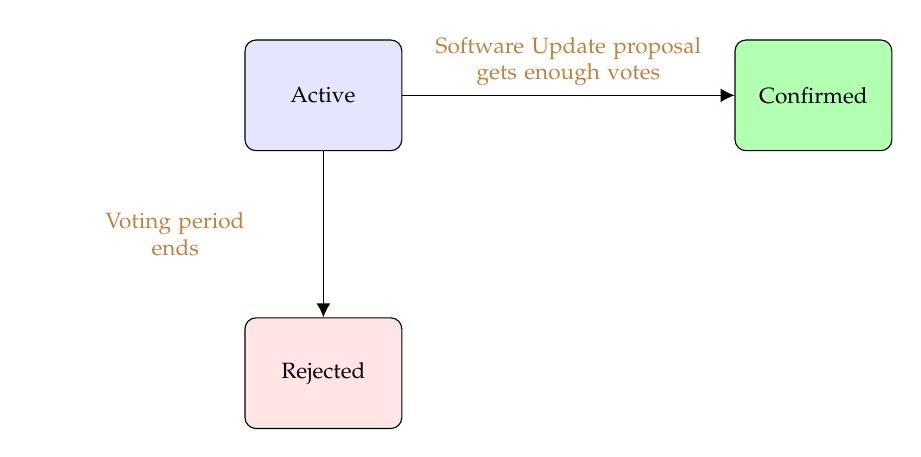
\begin{tikzpicture}[ align = center
                     , node distance = 6em and 12em
                     , text width = 5em
                     , font = \footnotesize
                     , >={Latex[width=0.5em, length=0.5em]}
                     , every node/.style = { rectangle
                                         , rounded corners
                                         , draw = black
                                         , align = center
                                         , minimum height = 4em }
                     ]

  \node (active) [fill = blue!10] {Active};
  \node (rejected) [below = of active, fill = red!10] {Rejected};
  \node (confirmed) [right = of active, fill = green!30] {Confirmed};

  \tikzset{every node/.style={align=center, text width=10em, text=brown}}

  \draw[->] (active)
  edge node [above] {Software Update proposal\\ gets enough votes}
  (confirmed);

  \draw[->] (active)
  edge node [left] {Voting period \\ends}
  (rejected);

  \end{tikzpicture}

  \caption{State-transition diagram for software-updates}
  \label{fig:st-diagram-sw-up}
\end{figure}

\clearpage

The interface rule for protocol-version endorsement makes use of the
$\trans{upend}{}$ transition, where we set the threshold for proposal adoption
to: the number of genesis keys ($\var{ngk}$) times the minimum proportion of
genesis keys that need to endorse an update proposal for it to become a
candidate for adoption (given by the protocol parameter $\var{upAdptThd}$). In
addition, the unconfirmed proposals that are older than $u$ blocks are removed
from the parts of the state that hold:
\begin{itemize}
\item the registered protocol and software update proposals,
\item the votes associated with the proposals,
\item the set of endorsement-key pairs, and
\item the block number in which proposals where added.
\end{itemize}

In Rule~\ref{eq:rule:upi-pend}, the set of proposal id's $\var{pid_{keep}}$
contains only those proposals that haven't expired yet or that are confirmed.
Once a proposal $\var{up}$ is confirmed, it is removed from the set of
confirmed proposals ($\var{cps}$) when a new a protocol version gets adopted
(see Rule~\ref{eq:rule:upi-ec-pv-change}).
%
The set of endorsement-key pairs is cleaned here as well as in the epoch change
rule (Rule~\ref{eq:rule:upi-ec-pv-change}). The reason for this is that this set grows at
each block, and it can get considerably large if no proposal gets adopted at
the end on an epoch.

\begin{figure}[htb]
  \begin{equation}
    \label{eq:rule:upi-pend}
    \inference
    {
      {
        \begin{array}{l}
          k\\
          s_n\\
          q \cdot \var{ngk}\\
          \var{dms}\\
          \var{cps}\\
          \var{rpus}
        \end{array}
      }
      \vdash
      {
        \left(
          \begin{array}{l}
            \var{fads}\\
            \var{bvs}
          \end{array}
        \right)
      }
      \trans{upend}{(\var{bv}, \var{vk})}
      {
        \left(
          \begin{array}{l}
            \var{fads'}\\
            \var{bvs'}
          \end{array}
        \right)
      }\\
      \var{stableAfter} \mapsto k \in  \var{pps}
      & \var{upropTTL} \mapsto u \in \var{pps}
      & \var{upAdptThd} \mapsto q \in \var{pps} \\
      {
        \begin{array}{r@{~\leteq~}l}
          \var{pids_{keep}} & \dom~(pws \restrictrange [s_n - u, ..]) \cup \dom~\var{cps}\\
          \var{vs_{keep}} & \dom~(\range~\var{rpus'})\\
          \var{rpus'} & \var{pids_{keep}} \restrictdom \var{rpus}
        \end{array}
      }
    }
    {
      {
        \begin{array}{l}
          s_n\\
          \var{ngk}\\
          \var{dms}
        \end{array}
      }
      \vdash
      {
        \left(
          \begin{array}{l}
            \var{e_p}\\
            (\var{pv}, \var{pps})\\
            \var{fads}\\
            \var{avs}\\
            \var{rpus}\\
            \var{raus}\\
            \var{cps}\\
            \var{vts}\\
            \var{bvs}\\
            \var{pws}
          \end{array}
        \right)
      }
      \trans{upiend}{(\var{bv}, \var{vk})}
      {
        \left(
          \begin{array}{l}
            \var{e_p}\\
            (\var{pv}, \var{pps})\\
            \var{fads'}\\
            \var{avs}\\
            \var{rpus'}\\
            \var{pids_{keep}} \restrictdom \var{raus}\\
            \var{cps}\\
            \var{pids_{keep}} \restrictdom \var{vts}\\
            \var{vs_{keep}}  \restrictdom \var{bvs'}\\
            \var{pids_{keep}} \restrictdom \var{pws}
          \end{array}
        \right)
      }
    }
  \end{equation}
  \caption{Proposal endorsement rules}
  \label{fig:rules:upi-pend}
\end{figure}

\clearpage

Rule~\ref{eq:rule:upi-ec-pv-change} models how the epoch, protocol-version and its
parameters are changed depending on the epoch in the signal ($e_n$ in this
case). A change in the epoch only occurs if the new epoch is greater than the
previously seen epoch ($e_p$).
%
On an epoch change, this rule will pick a candidate that gathered enough
endorsements at least $2 \cdot k$ slots ago. If a protocol-version candidate
cannot gather enough endorsements $2 \cdot k$ slots before the end of an
epoch, the proposal can only be adopted in the next epoch.
%
Figure~\ref{fig:up-confirmed-too-late} shows an example of a proposal being
confirmed too late in an epoch, where it is not possible to get enough
endorsements in the remaining window. In this Figure we take $k = 2$, and we
assume $4$ endorsements are needed to consider a proposal as candidate for
adoption.
%
Note that, in the final state, we use union override to define the updated
parameters ($\var{pps} \unionoverrideRight \var{pps'}$). This is because candidate
proposal might only update some parameters of the protocol.

In Rule~\ref{eq:rule:upi-ec-pv-change}, when a new proposal gets adopted, all
the state components that refer to protocol update proposals get emptied. The
reason for this is that at the moment of registering a proposal, we evaluated
it in a state where the protocol parameters that we used for this are no longer
up to date (see for instance \cref{eq:func:can-update}). For instance, assume
we register a proposal $\var{up}$ which only changes the maximum transaction
size to $x$, and the current block size is set to $x + 1$. Then,
$\fun{canUpdate}$ holds, since the maximum transaction size is less than the
maximum block size. If now a new proposal gets adopted that changes the maximum
block size to $x - 1$, then this invalidates $\var{up}$ since $\fun{canUpdate}$
no longer holds.
%

If there are no candidates for adoption, then the state variables remain
unaltered (Rule~\ref{eq:rule:upi-ec-pv-unchanged}).

Also note that the registered software-update proposals need not be cleaned
here, since this is done either when a proposal gets confirmed or when it
expires.

\begin{figure}[htb]
  \begin{equation}
    \label{eq:rule:pvbump-change-noop}
    \inference
    {
      e_n \leq e_p
    }
    {
      {\begin{array}{l}
         k\\
         s_n\\
         \var{fads}
       \end{array}}
      \vdash
      {
        \left(
          \begin{array}{l}
            \var{e_p}\\
            \var{(\var{pv}, \var{pps})}
          \end{array}
        \right)
      }
      \trans{pvbump}{\var{e_n}}
      {
        \left(
          \begin{array}{l}
            \var{e_p}\\
            \var{(\var{pv}, \var{pps})}
          \end{array}
        \right)
      }
    }
  \end{equation}
  \nextdef
  \begin{equation}
    \label{eq:rule:pvbump-change-epoch-only}
    \inference
    {
      [.., s_n - 2 \cdot k] \restrictdom \var{fads} = \epsilon &  e_p < e_n
    }
    {
      {\begin{array}{l}
         k\\
         s_n\\
         \var{fads}
       \end{array}}
      \vdash
      {
        \left(
          \begin{array}{l}
            \var{e_p}\\
            \var{(\var{pv}, \var{pps})}\\
          \end{array}
        \right)
      }
      \trans{pvbump}{\var{e_n}}
      {
        \left(
          \begin{array}{l}
            \var{e_n}\\
            \var{(\var{pv}, \var{pps})}\\
          \end{array}
        \right)
      }
    }
  \end{equation}
  \nextdef
  \begin{equation}
    \label{eq:rule:pvbump-change}
    \inference
    {
      \wcard ; (\wcard , (\var{pv_c}, \var{pps_c})) \leteq [.., s_n - 2 \cdot k] \restrictdom \var{fads}
      & e_p < e_n
    }
    {
      {\begin{array}{l}
         k\\
         s_n\\
         \var{fads}
       \end{array}}
      \vdash
      {
        \left(
          \begin{array}{l}
            \var{e_p}\\
            \var{(\var{pv}, \var{pps})}\\
          \end{array}
        \right)
      }
      \trans{pvbump}{\var{e_n}}
      {
        \left(
          \begin{array}{l}
            \var{e_n}\\
            \var{(\var{pv_c}, \var{pps_c})}\\
          \end{array}
        \right)
      }
    }
  \end{equation}
  \caption{Protocol version bump rules}
  \label{fig:rules:fads}
\end{figure}

\begin{figure}[htb]
  \begin{equation}
    \label{eq:rule:upi-ec-pv-unchanged}
    \inference
    {
      \var{stableAfter} \mapsto k \in  \var{pps} &
      {\begin{array}{l}
         k\\
         s_n\\
         \var{fads}
       \end{array}}
      \vdash
      {
        \left(
          \begin{array}{l}
            \var{e_p}\\
            \var{(\var{pv}, \var{pps})}
          \end{array}
        \right)
      }
      \trans{pvbump}{\var{e_n}}
      {
        \left(
          \begin{array}{l}
            \var{e'}\\
            \var{(\var{pv'}, \var{pps'})}\\
          \end{array}
        \right)
      }\\ ~ \\ \var{pv} = \var{pv'}
    }
    {
      {
        \begin{array}{l}
          s_n\\
          \var{ngk}\\
          \var{dms}
        \end{array}
      }
      \vdash
      {
        \left(
          \begin{array}{l}
            \var{e_p}\\
            \var{(\var{pv}, \var{pps})}\\
            \var{fads}\\
            \var{avs}\\
            \var{rpus}\\
            \var{raus}\\
            \var{cps}\\
            \var{vts}\\
            \var{bvs}\\
            \var{pws}
          \end{array}
        \right)
      }
      \trans{upiec}{\var{e_n}}
      {
        \left(
          \begin{array}{l}
            \var{e'}\\
            \var{(\var{pv}, \var{pps})}\\
            \var{fads}\\
            \var{avs}\\
            \var{rpus}\\
            \var{raus}\\
            \var{cps}\\
            \var{vts}\\
            \var{bvs}\\
            \var{pws}
          \end{array}
        \right)
      }
    }
  \end{equation}
  \nextdef
  \begin{equation}
    \label{eq:rule:upi-ec-pv-change}
    \inference
    {
      \var{stableAfter} \mapsto k \in  \var{pps} &
      {\begin{array}{l}
         k\\
         s_n\\
         \var{fads}
       \end{array}}
      \vdash
      {
        \left(
          \begin{array}{l}
            \var{e_p}\\
            \var{(\var{pv}, \var{pps})}
          \end{array}
        \right)
      }
      \trans{pvbump}{\var{e_n}}
      {
        \left(
          \begin{array}{l}
            \var{e'}\\
            \var{(\var{pv'}, \var{pps'})}\\
          \end{array}
        \right)
      }\\ ~ \\ \var{pv} \neq \var{pv'}
    }
    {
      {
        \begin{array}{l}
          s_n\\
          \var{ngk}\\
          \var{dms}
        \end{array}
      }
      \vdash
      {
        \left(
          \begin{array}{l}
            \var{e_p}\\
            \var{(\var{pv}, \var{pps})}\\
            \var{fads}\\
            \var{avs}\\
            \var{rpus}\\
            \var{raus}\\
            \var{cps}\\
            \var{vts}\\
            \var{bvs}\\
            \var{pws}
          \end{array}
        \right)
      }
      \trans{upiec}{\var{e_n}}
      {
        \left(
          \begin{array}{l}
            \var{e'}\\
            \var{(\var{pv'}, \var{pps'})}\\
            \epsilon\\
            \var{avs}\\
            \emptyset\\
            \var{raus}\\
            \emptyset\\
            \emptyset\\
            \emptyset\\
            \emptyset\\
          \end{array}
        \right)
      }
    }
  \end{equation}
  \caption{Block version adoption on epoch change rules}
  \label{fig:rules:upi-ec}
\end{figure}

\begin{figure}[htb]
  \centering
  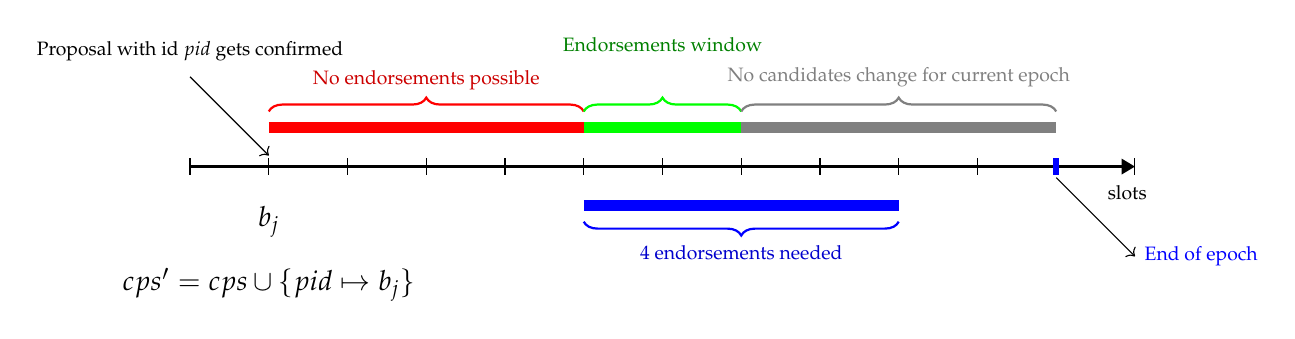
\begin{tikzpicture}
    %%
    %% Macros used in this picture
    %%
    %
    % Number of slots
    \pgfmathsetmacro{\nrSlots}{12}
    % Slot in which the proposal gets confirmed
    \pgfmathsetmacro{\cSlot}{1}
    % Our special K.
    \pgfmathsetmacro{\K}{4}
    % Epoch end.
    \pgfmathsetmacro{\eend}{11}
    % Number of positive votes needed
    \pgfmathsetmacro{\votes}{4}

    % Draw the horizontal line
    \draw[thick, -Triangle] (0,0) -- (\nrSlots,0)
    node[font=\scriptsize,below left=3pt and -8pt]{slots};

    % % draw vertical lines
    \foreach \x in {0,1,...,\nrSlots}
    \draw (\x cm, 3pt) -- (\x cm, -3pt);

    % Add a label to with the block number in which the proposal got confirmed.
    \node at (\cSlot, -.7) {$b_j$};

    % Update in cps
    \node at (\cSlot, -1.5) {$\var{cps'} = \var{cps} \cup \{ \var{pid} \mapsto b_j \}$};

    % The no-endorsements red bar.
    \draw[red, line width=4pt] (\cSlot, .5) -- +(\K, 0);

    % Brace above the no-endorsement window bar.
    \draw[thick, red, decorate, decoration={brace, amplitude=5pt}]
    (\cSlot, .7) -- +(\K, 0)
    node[black!20!red, midway, above=4pt, font=\scriptsize] {No endorsements possible};

    % The endorsements window.
    \coordinate (ewStart) at (\cSlot + \K, .5);
    \coordinate (ewEnd) at ($(\eend - \K, .5)$);
    \draw[green, line width=4pt]
    (ewStart) -- (ewEnd);

    % Brace above the endorsements window
    \coordinate (ewStartB) at ($(ewStart) + (0, 0.2)$);
    \coordinate (ewEndB) at ($(ewEnd) + (0, 0.2)$);
    \draw[thick, green, decorate, decoration={brace, amplitude=5pt}]
    (ewStartB) -- (ewEndB)
    node[black!50!green, midway, above=18pt, font=\scriptsize] {Endorsements window};

    % The no-candidates change window.
    \coordinate (nccStart) at (\eend - \K, .5);
    \coordinate (nccEnd) at ($(\eend, .5)$);
    \draw[gray, line width=4pt]
    (nccStart) -- (nccEnd);

    % Brace above the no-candidates change window.
    \coordinate (nccStartB) at ($(nccStart) + (0, 0.2)$);
    \coordinate (nccEndB) at ($(nccEnd) + (0, 0.2)$);
    \draw[thick, gray, decorate, decoration={brace, amplitude=5pt}]
    (nccStartB) -- (nccEndB)
    node[gray, midway, above=5pt, font=\scriptsize] {No candidates change for current epoch};


    % The 2k before end-of-epoch window.
    \coordinate (beeStart) at (\cSlot + \K, -.5);
    \coordinate (beeEnd) at ($(\cSlot + \K + \votes, -.5)$);
    \draw[blue, line width=4pt]
    (beeStart) -- (beeEnd);

    % Brace on above the 2k before end-of-epoch window.
    \coordinate (beeStartB) at ($(beeStart) - (0, 0.2)$);
    \coordinate (beeEndB) at ($(beeEnd) - (0, 0.2)$);
    \draw[thick, blue, decorate, decoration={brace, amplitude=5pt}]
    (beeEndB) -- (beeStartB)
    node[black!20!blue, midway, below=5pt, font=\scriptsize] {$\votes$ endorsements needed};

    \draw[blue, line width=2pt] (\eend, 3pt) -- (\eend, -3pt);

    \draw[<-] (\cSlot, 4pt) -- +(-1, 1)
    node [above=2pt, black, font=\scriptsize]
    {Proposal with id $\var{pid}$ gets confirmed};

    \draw[->] (\eend, -4pt) -- +(1, -1)
    node[right, blue, font=\scriptsize] {End of epoch};
  \end{tikzpicture}
  \caption{An update proposal confirmed too late}
  \label{fig:up-confirmed-too-late}
\end{figure}

Figure~\ref{fig:st-diagram-pt-up} shows the different states a protocol-update
proposal can be in, and what causes the transitions between them.

\begin{figure}[ht]
  \centering
  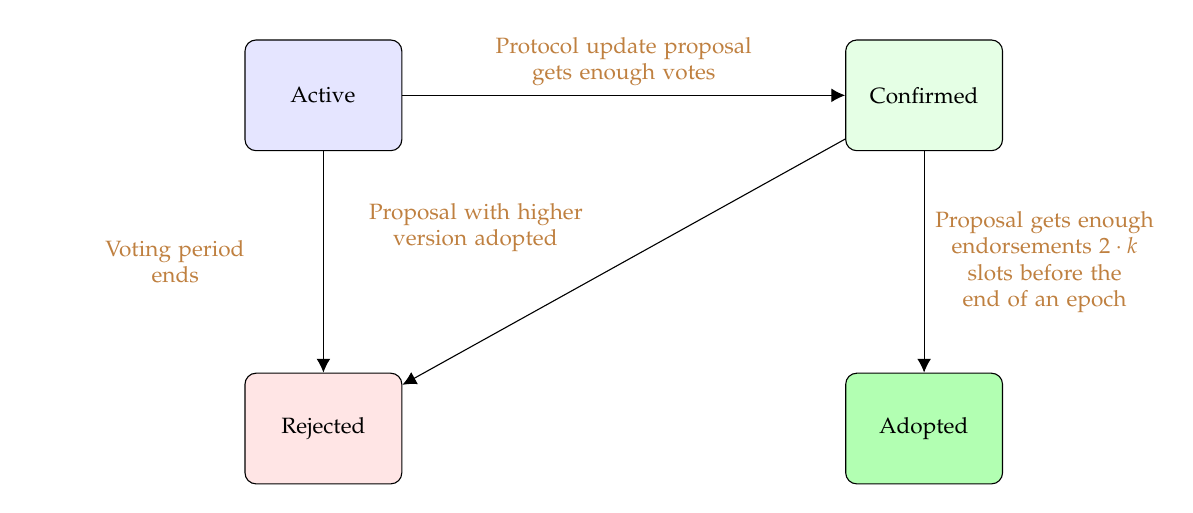
\begin{tikzpicture}[ align = center
                     , node distance = 8em and 16em
                     , text width = 5em
                     , font = \footnotesize
                     , >={Latex[width=0.5em, length=0.5em]}
                     , every node/.style = { rectangle
                                         , rounded corners
                                         , draw = black
                                         , align = center
                                         , minimum height = 4em }
                     ]

  \node (active) [fill = blue!10] {Active};
  \node (rejected) [below = of active, fill = red!10] {Rejected};
  \node (confirmed) [right = of active, fill = green!10] {Confirmed};
  \node (adopted) [below = of confirmed, fill = green!30] {Adopted};

  \tikzset{every node/.style={align=center, text width=10em, text=brown}}

  \draw[->] (active)
  edge node [above] {Protocol update proposal\\ gets enough votes}
  (confirmed);

  \draw[->] (active)
  edge node [left] {Voting period \\ends}
  (rejected);

  \draw[->] (confirmed)
  edge node [above left]
  {Proposal with higher version adopted}
  (rejected);

  \draw[->] (confirmed)
  edge node [right, text width=8em]
  {Proposal gets enough endorsements $2 \cdot k$ slots before the end of an epoch}
  (adopted);

  \end{tikzpicture}

  \caption{State-transition diagram for protocol-updates}
  \label{fig:st-diagram-pt-up}
\end{figure}


In this section we discuss the properties which we want the ledger to have. One
goal is to include these properties in the executable specification for doing
property-based testing or formal verification.

\subsection{Validity of a Ledger State}
\label{sec:valid-ledg-state}

Many properties only make sense when applied to a valid ledger state. In
informal terms, a valid ledger state $l$ can only be reached when starting from
an initial state $l_{0}$ (genesis state) and only executing state transition
rules as specified in Section~\ref{sec:state-trans-utxo-1} for UTxO or
Section~\ref{sec:delegation} for delegation.

\begin{figure}[ht]
  \centering
  \begin{align*}
    \genesisId & \in & \TxId \\
    \genesisTxOut & \in & \TxOut \\
    \genesisUTxO & \coloneqq & \{\genesisId, \emptyset\} \mapsto \genesisTxOut
    \\
    \ledgerState & \in & \left(
                         \begin{array}{c}
                           \UTxO \\
                           \DPState
                         \end{array}
    \right)\\
               && \\
    \fun{getUTxO} & \in & \ledgerState \to \UTxO \\
    \fun{getUTxO} & \coloneqq & (\var{utxo}, \wcard) \to \var{utxo}
  \end{align*}
  \caption{Definitions and Functions for Valid Ledger State}
  \label{fig:valid-ledger}
\end{figure}

In Figure~\ref{fig:valid-ledger} \genesisId{} marks the transaction identifier
of the initial coin distribution, where \genesisTxOut{} represents the initial
UTxO. It should be noted that no corresponding inputs exists, i.e., the
transaction inputs are the empty set for the initial transaction. An element of
\ledgerState{} is a tuple of UTxO and delegation witness state (\DPState).

\begin{definition}[\textbf{Valid Ledger State}]
  \begin{multline*}
    \forall l_{0},\ldots,l_{n} \in \ledgerState, l_{0} =
    \left(
      \begin{array}{c}
        \left\{
        \genesisUTxO
        \right\} \\
        \left(
        \begin{array}{c}
          \emptyset\\
          \emptyset
        \end{array}
        \right)
      \end{array}
    \right)  \\
    \implies \forall 0 < i \leq n, (\exists tx_{i} \in \Tx, l_{i-1}
    \trans{ledger}{tx_{i}} l_{i}) \implies \applyFun{validLedgerState} l_{n}
  \end{multline*}
  \label{def:valid-ledger-state}
\end{definition}

Definition~\ref{def:valid-ledger-state} defines a valid ledger state reachable
from the genesis state via valid UTxO, stake delegation or stake pool
transactions. This gives a constructive rule how to reach a valid ledger state.

\subsection{Ledger Properties}
\label{sec:ledger-properties}

The following properties state the desired features of updating a valid ledger
state.

\begin{property}[\textbf{Preserve Balance Modulo Fee}]
  \begin{multline*}
    \forall \var{l}, \var{l'} \in \ledgerState: \applyFun{validLedgerstate}{l}\\
    \implies \forall \var{tx} \in \Tx, \var{l} \trans{utxow}{tx} \var{l'} \\
    \implies \applyFun{destroyed}{pc utxo stKeys rewards tx} =
    \applyFun{created}{pc stPools tx}
  \end{multline*}
  \label{prop:ledger-properties-1}
\end{property}

Property~\ref{prop:ledger-properties-1} states that for each valid ledger $l$,
if a transaction $tx$ is added to the ledger via the state transition rule
$utxow$ to the new ledger state $l'$, the balance of the UTxOs in $l$ equals the
balance of the UTxOs in $l'$ in the sense that the amount of created value in
$l'$ equals the amount of destroyed value in $l$. This means that the total
amount of value is left unchanged by a transaction.

\begin{property}[\textbf{Preserve Balance Restricted to TxIns in Balance of
    TxOuts}]
  \begin{multline*}
    \forall \var{l}, \var{l'} \in \ledgerState: \applyFun{validLedgerstate}{l}\\
    \implies \forall \var{tx} \in \Tx, \var{l} \trans{utxow}{tx} \var{l'}
    \implies \fun{balance}(\applyFun{txins}{tx} \restrictdom
    \applyFun{getUTxO}{l}) = \fun{balance}(\applyFun{outs}{tx}) +
    \applyFun{txfee}{tx}
  \end{multline*}
  \label{prop:ledger-properties-2}
\end{property}

Property~\ref{prop:ledger-properties-2} states the more detailed relation of the
balances change. For ledgers $l, l'$ and a transaction $tx$ as above, the
balance of the UTxOs of $l$ restricted to those whose domain is in the set of
transaction inputs of $tx$ equals the balance of the transaction outputs of $tx$
minus the transaction fees.

\begin{property}[\textbf{Preserve Outputs of Transaction}]
  \begin{multline*}
    \forall \var{l}, \var{l'} \in \ledgerState: \applyFun{validLedgerstate}{l}\\
    \implies \forall \var{tx} \in \Tx, \var{l} \trans{utxow}{tx} \var{l'}
    \implies \forall \var{out} \in \applyFun{outs}{tx}, out \in
    \applyFun{getUTxO}{l'}
  \end{multline*}
  \label{prop:ledger-properties-3}
\end{property}

Property~\ref{prop:ledger-properties-3} states that for every ledger states
$l, l'$ and transaction $tx$ as above, all output UTxOs of $tx$ are in the UTxO
set of $l'$, i.e., they are now available as unspent transaction output.

\begin{property}[\textbf{Eliminate Inputs of Transaction}]
  \begin{multline*}
    \forall \var{l}, \var{l'} \in \ledgerState: \applyFun{validLedgerstate}{l}\\
    \implies \forall \var{tx} \in \Tx, \var{l} \trans{utxow}{tx} \var{l'}
    \implies \forall \var{in} \in \applyFun{txins}{tx}, in \not\in
    \fun{dom}(\applyFun{getUTxO}{l'})
  \end{multline*}
  \label{prop:ledger-properties-4}
\end{property}

Property~\ref{prop:ledger-properties-4} states that for every ledger states
$l, l'$ and transaction $tx$ as above, all transaction inputs $in$ of $tx$ are
not in the domain of the UTxO set of $l'$, i.e., these are no longer available
to spend.

\begin{property}[\textbf{Completeness and Collision-Freeness of new Transaction
    Ids}]
  \begin{multline*}
    \forall \var{l}, \var{l'} \in \ledgerState: \applyFun{validLedgerstate}{l}\\
    \implies \forall \var{tx} \in \Tx, \var{l} \trans{utxow}{tx} \var{l'}
    \implies \forall utxo' \in \applyFun{outs}{tx}, \var{utxo'} \in
    \applyFun{getUTxO}{l'} \wedge \\(\var{utxo'} = ((\var{txId'}, \wcard) \mapsto
    \wcard) \implies \forall \var{utxo} \in \applyFun{getUTxO}{l}, \var{utxo} =
    ((\var{txId}, \wcard) \mapsto \wcard) \implies \var{txId'} \neq \var{txId}
  \end{multline*}
  \label{prop:ledger-properties-5}
\end{property}

Property~\ref{prop:ledger-properties-5} states that for ledger states $l, l'$
and a transaction $tx$ as above, the UTxOs of $l'$ contain all newly created
UTxOs and the referred transaction id of each new UTxO is not used in the UTxO
set of $l$.

\begin{property}[\textbf{Absence of Double-Spend}]
  \begin{multline*}
    \forall l_{0},\ldots,l_{n} \in \ledgerState, l_{0} =
    \left(
      \begin{array}{c}
        \left\{
        \genesisUTxO
        \right\} \\
        \left(
        \begin{array}{c}
          \emptyset\\
          \emptyset
        \end{array}
        \right)
      \end{array}
    \right) \wedge \applyFun{validLedgerState} l_{n} \\
    \implies \forall 0 < i \leq n, tx_{i} \in \Tx, l_{i-1}
    \trans{ledger}{tx_{i}} l_{i} \wedge \applyFun{validLedgerState} l_{i}
    \\ \implies \forall j < i, \applyFun{txins}{tx_{j}} \cap
    \applyFun{txins}{tx_{i}} = \emptyset
  \end{multline*}
  \label{prop:ledger-properties-no-double-spend}
\end{property}

Property~\ref{prop:ledger-properties-no-double-spend} states that for each valid
ledger state $l_{n}$ reachable from the genesis state, each transaction $t_{i}$
does not share any input with any previous transaction $t_{j}$. This means that
each output of a transition is spent at most once.

\subsection{Ledger State Properties for Delegation Transitions}
\label{sec:ledg-prop-deleg}

\begin{figure}[ht]
  \centering
  \begin{align*}
    \fun{getStKeys} & \in & \ledgerState \to \powerset \HashKey \\
    \fun{getStKeys} & \coloneqq & (\wcard, (\var{stKeys}, \wcard, \wcard),
                                  \wcard) \to \var{stkeys} \\
                    &&\\
    \fun{getRewards} & \in & \ledgerState \to \AddrRWD \mapsto \Coin \\
    \fun{getRewards} & \coloneqq & (\wcard, (\wcard, \var{rewards}, \wcard),
                                   \wcard) \to \var{rewards} \\
                    &&\\
    \fun{getDelegations} & \in & \ledgerState \to \HashKey \mapsto \HashKey \\
    \fun{getDelegations} & \coloneqq & (\wcard, (\wcard, \wcard,
                                       \var{delegations}), \wcard) \to
                                       \var{delegations} \\
                    &&\\
    \fun{getStPools} & \in & \ledgerState \to \HashKey \mapsto \DCertRegPool \\
    \fun{getStPools} & \coloneqq & (\wcard, \wcard,
                                   (\var{stpools}, \wcard)) \to \var{stpools} \\
                    &&\\
    \fun{getRetiring} & \in & \ledgerState \to \HashKey \mapsto \Epoch \\
    \fun{getRetiring} & \coloneqq & (\wcard, \wcard,
                                    (\wcard, \var{retiring})) \to \var{retiring} \\
  \end{align*}
  \caption{Definitions and Functions for Stake Delegation in Ledger States}
  \label{fig:stake-delegation-functions}
\end{figure}


\begin{property}[\textbf{Registered Staking Key with Zero Rewards}]
  \begin{multline*}
    \forall \var{l}, \var{l'} \in \ledgerState: \applyFun{validLedgerstate}{l}\\
    \implies \forall \var{c} \in \DCertRegKey, \var{l} \trans{delegw}{c} \var{l'}
    \implies \applyFun{author}{c} = \var{hk}\\ \implies
    \var{hk} \in \applyFun{getStKeys}{l'} \wedge
    (\applyFun{getRewards}var{rewards})[hk] = 0
  \end{multline*}
  \label{prop:ledger-properties-6}
\end{property}

Property~\ref{prop:ledger-properties-6} states that for each valid ledger state
$l$, if a delegation transaction of type $\DCertRegKey$ is executed, then in the
resulting ledger state $l'$, the set of staking keys of $l'$ includes the key
$hk$ associated with the key registration certificate and the associated reward
is set to 0 in $l'$.

\begin{property}[\textbf{Deregistered Staking Key}]
  \begin{multline*}
    \forall \var{l}, \var{l'} \in \ledgerState: \applyFun{validLedgerstate}{l}\\
    \implies \forall \var{c} \in \DCertDeRegKey, \var{l} \trans{delegw}{c} \var{l'}
    \implies \applyFun{author}{c} = \var{hk}\\ \implies
    \var{hk} \not\in \applyFun{getStKeys}{l'} \wedge
    (\fun{dom}(\applyFun{getRewards}{l'}) \cup
    \fun{dom}(\applyFun{getDelegations}{l'})) \cap \{hk\} = \emptyset
  \end{multline*}
  \label{prop:ledger-properties-7}
\end{property}

Property~\ref{prop:ledger-properties-7} states that for $l, l'$ as above but
with a delegation transition of type $\DCertDeRegKey$, the staking key $hk$
associated with the deregistration certificate is not in the set of staking keys
of $l'$ and is not in the domain of neither the rewards nor the delegation map
of $l'$.

\begin{property}[\textbf{Delegated Stake}]
  \begin{multline*}
    \forall \var{l}, \var{l'} \in \ledgerState: \applyFun{validLedgerstate}{l}\\
    \implies \forall \var{c} \in \DCertDeleg, \var{l} \trans{delegw}{c} \var{l'}
    \implies \applyFun{author}{c} = \var{hk}\\ \implies
    \var{hk} \in \applyFun{getStKeys}{l} \wedge
    (\applyFun{getDelegations}{l'})[hk] = \applyFun{pool}{c}
  \end{multline*}
  \label{prop:ledger-properties-8}
\end{property}

Property~\ref{prop:ledger-properties-8} states that for $l, l'$ as above but
with a delegation transition of type $\DCertDeleg$, the staking key $hk$
associated with the deregistration certificate is in the set of staking keys of
$l$ and delegates to the staking pool associated with the delegation
certificate in $l'$.

\subsection{Ledger State Properties for Staking Pool Transitions}
\label{sec:ledg-state-prop}

\begin{property}[\textbf{Registered Staking Pool}]
  \begin{multline*}
    \forall \var{l}, \var{l'} \in \ledgerState: \applyFun{validLedgerstate}{l}\\
    \implies \forall \var{c} \in \DCertRegPool, \var{l} \trans{pool}{c} \var{l'}
    \implies \applyFun{author}{c} = \var{hk}\\ \implies
    (\applyFun{getStPools}{l'})[\var{hk}] = c \wedge \var{hk} \not\in
    \applyFun{getRetiring}{l'}
  \end{multline*}
  \label{prop:ledger-properties-9}
\end{property}

Property~\ref{prop:ledger-properties-9} states that for $l, l'$ as above but
with a delegation transition of type $\DCertRegPool$, the key $hk$ is associated
with the author of the pool registration certificate in $\var{stpools}$ of $l'$
and that $hk$ is not in the set of retiring stake pools in $l'$.

\begin{property}[\textbf{Start Staking Pool Retirement}]
  \begin{multline*}
    \forall \var{l}, \var{l'} \in \ledgerState, \var{cepoch} \in \Epoch:
    \applyFun{validLedgerstate}{l} \\
    \implies \forall \var{c} \in \DCertRetirePool, \var{l} \trans{pool}{c} \var{l'}
    \\ \implies e = \applyFun{retire}{c} \wedge
    \var{cepoch} < e < \var{cepoch} + \emax \wedge \applyFun{author}{c} =
    \var{hk}\\ \implies (\applyFun{getRetiring}{l'})[\var{hk}] = e \wedge
    \var{hk} \in \fun{dom}(\applyFun{getStPools}{l})
  \end{multline*}
  \label{prop:ledger-properties-10}
\end{property}

Property~\ref{prop:ledger-properties-10} states that for $l, l'$ as above but
with a delegation transition of type $\DCertRetirePool$, the key $hk$ is
associated with the author of the pool registration certificate in
$\var{stpools}$ of $l'$ and that $hk$ is not in the set of retiring stake pools
in $l'$.

\begin{property}[\textbf{Stake Pool Reaping}]
  \begin{multline*}
    \forall \var{l}, \var{l'} \in \ledgerState, \var{cepoch} \in \Epoch:
    \applyFun{validLedgerstate}{l} \\
    \implies \var{l} \trans{poolreap}{} \var{l'} \implies \forall \var{retire} =
    retiring^{-1} cepoch, retired \neq \emptyset \\ \wedge \var{retire}
    \subseteq \fun{dom}(\applyFun{getStPool}{l}) \wedge
    \var{retire} \cap \fun{dom}(\applyFun{getStPool}{l'}) = \emptyset \\
    \wedge \var{retire} \subseteq \fun{dom}(\applyFun{getRetiring}{l}) \wedge
    \var{retire} \cap \fun{dom}(\applyFun{getRetiring}{l'}) = \emptyset
  \end{multline*}
  \label{prop:ledger-properties-11}
\end{property}

Property~\ref{prop:ledger-properties-11} states that for $l, l'$ as above but
with a delegation transition of type $\DPoolReap$, there exist registered stake
pools in $l$ which are associated to stake pool registration certificates and
which are to be retired at the current epoch $\var{cepoch}$. In $l'$ all those
stake pools are removed from the maps $stpools$ and $retiring$.


\subsection{Properties of Numerical Calculations}
\label{sec:prop-numer-calc}

The numerical calculations for refunds and rewards calculation in
(see Section~\ref{sec:epoch}) are also required to have certain properties. In
particular we need to make sure that the functions that use non-integral
arithmetic have properties which guarantee consistency of the system. Here, we
state those properties and formulate them in a way that makes them possible to
use properties-based testing for validation in the executable spec.

\begin{property}[\textbf{Minimal Refund}]
  \label{prop:minimal-refund}

  The function $\fun{refund}$ takes a value, a minimal percentage, a decay
  parameter and a duration. It must guarantee that the refunded amount is within
  the minimal refund (off-by-one for rounding / floor) and the original value.

  \begin{multline*}
    \forall d_{val} \in \mathbb{N}, d_{min} \in [0,1], \lambda \in (0, \infty),
    \delta \in \mathbb{N} \\
    \implies \max(0,d_{val}\cdot d_{min} - 1) \leq \floor*{d_{val}\cdot(d_{min} +
      (1-d_{min})\cdot e^{-\lambda\cdot\delta})} \leq d_{val}
  \end{multline*}
\end{property}


\begin{property}[\textbf{Exponential Moving Average}]
  \label{prop:exponential-moving-average}

  The function $\fun{movingAvg}$ calculates the exponential moving average,
  dividing the number of blocks created by the pool by the expected number of
  slots the pool is elected leader (or 1 if the expected number is below 1). It
  guarantees that the result is (i) non-negative and (ii) if a previous moving
  average has already been calculated, the new moving average lies between the
  minimum and maximum of the old and new calculated value. With
  $current := \frac{n}{\max(\overline{N}, 1)}$ this is trivial for (i), for (ii)
  it is

  \begin{multline*}
    \forall \alpha \in [0, 1], n \in \mathbb{N}, \overline{N} \in \Rnn, prev \in
    \Rnn\\
    \implies 0\leq \min(prev, current) \leq
    \alpha\cdot current + (1 - \alpha)\cdot prev
    \leq \max(prev, current)
  \end{multline*}
\end{property}

\begin{property}[\textbf{Actual Reward}]
  \label{prop:actual-reward}

  The actual reward for a stake pool in an epoch is calculated by the function
  $\fun{poolReward}$. The actual reward per stake pool is non-negative and
  bounded by the maximal reward for the stake pool, with $avg$ being the
  calculated moving average of the stake pool and $maxP$ being the maximal
  reward for the stake pool, we get:

  \begin{equation*}
    \forall \gamma \in [0,1] \implies 0\leq \floor*{avg^{\gamma}\cdot maxP} \leq maxP
  \end{equation*}
\end{property}

\begin{todo}
  The property~(\ref{prop:actual-reward}) requires that $avg \in [0,1]$, else
  the actual reward can exceed the maximal reward. This is not true, we need to
  take into account the rewards for all stake pools.
\end{todo}


%%% Local Variables:
%%% mode: latex
%%% TeX-master: "ledger-spec"
%%% End:


\addcontentsline{toc}{section}{References}
\bibliographystyle{plainnat}
\bibliography{references}

\end{document}
